\documentclass[12pt,a4paper]{article}
%
%	STARWARE - Stile base per la scrittura di documenti interni in LaTex
%

%
%	Pacchetti globali
%	Fare qui eventuali aggiunte!
%
\usepackage[utf8]{inputenc}
\usepackage[italian]{babel}
\usepackage[babel]{csquotes}
\usepackage{url}
\usepackage{graphicx}
\usepackage[colorlinks]{hyperref}
\usepackage{lastpage}
\usepackage{fancyhdr}
\usepackage[top=1cm,bottom=4cm,left=80pt,right=80pt]{geometry} %disegna la linea
\usepackage{listings} %per grandi porzioni di codice
\usepackage{color}
\usepackage[table]{xcolor}
\usepackage{booktabs,tabularx}
\usepackage{makeidx}
\usepackage{fixltx2e}
\usepackage{hyperref}
\usepackage{enumitem}
\usepackage{color}
\usepackage[T1]{fontenc}
\usepackage{float}
\usepackage{svg}
\usepackage{amsmath}
\usepackage[toc]{glossaries}
\usepackage{dirtree}
\usepackage{listings}

\makeglossaries

\bibliographystyle{alpha}

%
%	VARIABILI GLOBALI
%
\newcommand{\nomeGruppo}{StarWare}
\newcommand{\mailGruppo}{starware.swe@gmail.com}
\newcommand{\uni}{Universit\`{a} degli Studi di Padova}
\newcommand{\uniAA}{2015/2016}
\newcommand{\Cardin}{Prof. Riccardo Cardin}
\newcommand{\Vardanega}{Prof. Tullio Vardanega}
\newcommand{\Zucchetti}{Zucchetti S.p.a.}
\newcommand{\prj}{Quizzipedia}
\newcommand{\prjL}{Quizzipedia: software per la gestione di questionari}

\newcommand{\AVI}{Alessio Vitella}
\newcommand{\AVE}{Andrea Venier}
\newcommand{\NDC}{Nicola De Cao}
\newcommand{\IB}{Igor Baylyak}
\newcommand{\WS}{Walter Sandon}
\newcommand{\TP}{Thomas Pigarelli}
\newcommand{\AB}{Anna Bonaldo}

\newcommand{\mgls}[1]{\gls{#1}\textsubscript{G}}
\newcommand{\mglspl}[1]{\glspl{#1}\textsubscript{G}}
\newcommand{\mGls}[1]{\Gls{#1}\textsubscript{G}}
\newcommand{\mGlspl}[1]{\Glspl{#1}\textsubscript{G}}

\newcommand{\AM}{\emph{\mGls{amministratore}}}
\newcommand{\AN}{\emph{\mGls{analista}}}
\newcommand{\PG}{\emph{\mGls{progettista}}}
\newcommand{\PR}{\emph{\mGls{programmatore}}}
\newcommand{\VR}{\emph{\mGls{verificatore}}}
\newcommand{\PM}{\emph{\mGls{project manager}}}

\newcommand{\AMpl}{\emph{\mGlspl{amministratore}}}
\newcommand{\ANpl}{\emph{\mGlspl{analista}}}
\newcommand{\PGpl}{\emph{\mGlspl{progettista}}}
\newcommand{\PRpl}{\emph{\mGlspl{programmatore}}}
\newcommand{\VRpl}{\emph{\mGlspl{verificatore}}}
\newcommand{\PMpl}{\emph{\mGlspl{project manager}}}

\newcommand{\RR}{\emph{\mGls{revisione dei requisiti}}}
\newcommand{\RA}{\emph{\mGls{revisione di accettazione}}}
\newcommand{\RP}{\emph{\mGls{revisione di progettazione}}}
\newcommand{\RQ}{\emph{\mGls{revisione di qualifica}}}

\newcommand{\NdP}{\emph{\mGls{norme di progetto}}}
\newcommand{\SdF}{\emph{\mGls{stidio di fattibilita}}}
\newcommand{\AdR}{\emph{\mGls{analisi dei requisiti}}}
\newcommand{\PdP}{\emph{\mGls{piano di progetto}}}
\newcommand{\PdQ}{\emph{\mGls{piano di qualifica}}}

\newcommand{\latex}[1]{\texttt{#1}}
\newcommand{\fileName}[1]{\texttt{#1}}
\newcommand{\filePath}[1]{\texttt{#1}}
\newcommand{\TODO}[1]{\texttt{\large \color{red} \underline{TODO: #1}}}

\newcommand{\licenza}{GNU GENERAL PUBLIC LICENSE V2}

%per compilare il template usare questi sotto e commentare glia altri:
%\newcommand{\logoLungo}{../imgs/logoLungo.png}
%\newcommand{\logoGrande}{../imgs/logoGrande.png}
\newcommand{\logoLungo}{../../../template/imgs/logoLungo.png}
\newcommand{\logoGrande}{../../../template/imgs/logoGrande.png}

%
%	Setup stili
%

\newcommand{\HRule}{\rule{\linewidth}{0.5mm}}

\definecolor{dkgreen}{rgb}{0,0.6,0}
\definecolor{gray}{rgb}{0.5,0.5,0.5}
\definecolor{mauve}{rgb}{0.58,0,0.82}
\definecolor{light}{RGB}{255,255,190}

%
%	Setup di pagina
%

%colorazione link
\hypersetup
{
	colorlinks=true,
	linkcolor=black,
	urlcolor=blue,
	citecolor=blue
}

%	Setup Header + Footer

\pagestyle{fancy}
\setlength{\headheight}{2cm} %settato grandezza header

\renewcommand{\footrulewidth}{0.5pt} %ridefinisco il valore della riga di intestazione
\renewcommand{\headrulewidth}{0.5pt} %ridefinisco il valore della riga di pie' di pagina
\addtolength{\headwidth}{\marginparsep}
\addtolength{\headwidth}{\marginparwidth}

\fancyhead{} %annulla head di default
\fancyfoot{} %annulla foot di default

%	Logo intestazione
\lhead{
\includegraphics[scale=0.12]{\logoLungo}}


%	footer
\cfoot{
	\uni \ - \uniAA \\
	\href{mailto:\mailGruppo}{\mailGruppo}\\
	{\tiny Questo documento è distribuito sotto licenza {\licenza}}
}
\rfoot{
	\thepage\ di \pageref{LastPage}
}


% test subsubsubsection

\usepackage{titlesec}
\usepackage{hyperref}

\titleclass{\subsubsubsection}{straight}[\subsection]

\newcounter{subsubsubsection}[subsubsection]
\renewcommand\thesubsubsubsection{\thesubsubsection.\arabic{subsubsubsection}}
\renewcommand\theparagraph{\thesubsubsubsection.\arabic{paragraph}} % optional; useful if paragraphs are to be numbered

\titleformat{\subsubsubsection}
  {\normalfont\normalsize\bfseries}{\thesubsubsubsection}{1em}{}
\titlespacing*{\subsubsubsection}
{0pt}{3.25ex plus 1ex minus .2ex}{1.5ex plus .2ex}

\makeatletter
\renewcommand\paragraph{\@startsection{paragraph}{5}{\z@}%
  {3.25ex \@plus1ex \@minus.2ex}%
  {-1em}%
  {\normalfont\normalsize\bfseries}}
\renewcommand\subparagraph{\@startsection{subparagraph}{6}{\parindent}%
  {3.25ex \@plus1ex \@minus .2ex}%
  {-1em}%
  {\normalfont\normalsize\bfseries}}
\def\toclevel@subsubsubsection{4}
\def\toclevel@paragraph{5}
\def\toclevel@paragraph{6}
\def\l@subsubsubsection{\@dottedtocline{4}{7em}{4em}}
\def\l@paragraph{\@dottedtocline{5}{10em}{5em}}
\def\l@subparagraph{\@dottedtocline{6}{14em}{6em}}
\makeatother

\setcounter{secnumdepth}{4}
\setcounter{tocdepth}{4}


%pdflatex -synctex=1 -interaction=nonstopmode %.tex|makeglossaries %|pdflatex -synctex=1 -interaction=nonstopmode %.tex|pdflatex -synctex=1 -interaction=nonstopmode %.tex
\makeglossary

\newglossaryentry{responsabile} {
	name=responsabile,
	description={è il responsabile della gestione, pianificazione e realizzazione del progetto},
	plural=Responsabili
}

\newglossaryentry{verificatore} {
	name=verificatore,
	description={è il responsabile dell'attività di verifica},
	plural=Verificatori
}

\newglossaryentry{programmatore} {
	name=programmatore,
	description={è responsabile delle attività di codifica miranti alla realizzazione del prodotto e delle componenti di ausilio necessarie per l'esecuzione delle prove di verifica e validazione},
	plural=programmatori
}

\newglossaryentry{progettista} {
	name=progettista,
	description={è responsabile delle attività di progettazione},
	plural=Progettisti
}

\newglossaryentry{analista} {
	name=analista,
	description={è responsabile delle attività di analisi. },
	plural=Analisti
}

\newglossaryentry{amministratore} {
	name=amministratore,
	description={è responsabile dell'efficienza e dell'operatività dell'ambiente di sviluppo; si occupa della redazione e attuazione di piani e procedure di gestione della qualità; inoltre gestisce l'archivio della documentazione del progetto},
	plural=Amministratori
}

\newglossaryentry{revisione dei requisiti} {
	name=revisione dei requisiti,
	description={è una revisione formale che determina l'accesso del gruppo al progetto didattico e la concordanza con il cliente di una visione condivisa del prodotto atteso}
}

\newglossaryentry{revisione di accettazione} {
	name=revisione di accettazione,
	description={è una revisione formale per l'accertamento del soddisfacimento di tutti i requisiti e il completamento del progetto}
}

\newglossaryentry{revisione di progettazione} {
	name=revisione di progettazione,
	description={è una revisione di progresso che accerta la realizzabilità del prodotto e informa il cliente sulle caratteristiche del prodotto}
}

\newglossaryentry{revisione di qualifica} {
	name=revisione di qualifica,
	description={è una revisione di progresso che approva l'esito finale delle verifiche e attiva la fase di validazione}
}

\newglossaryentry{analisi} {
	name=analisi,
	description={è il periodo di preparazione e produzioni di documenti che precede la Revisione dei requisiti}
}

\newglossaryentry{progettazione} {
	name=progettazione,
	description={è il periodo che intercorre tra la Revisione dei requisiti e la Revisione di progettazione}
}

\newglossaryentry{codifica} {
	name=codifica,
	description={è il periodo che intercorre tra la Revisione di progettazione e la Revisione di qualifica}
}

\newglossaryentry{validazione} {
	name=validazione,
	description={è il periodo che intercorre tra la Revisione di qualifica e la Revisione di accettazione}
}

\newglossaryentry{repository} {
	name=repository,
	description={è dove i file sono memorizzati, spesso su un server}
}

\newglossaryentry{ruolo} {
	name=ruolo,
	description={una delle figure professionali che una persona fisica interpreta nel corso del progetto. I ruoli sono: responsabile, amministratore, analista, progettista, programmatore e verificatore},
    plural=ruoli
}

\newglossaryentry{svg} {
	name=SVG,
	description={è un formato per la visualizzazione di oggetti in grafica vettoriale. Per maggiori informazioni si veda \href{https://it.wikipedia.org/wiki/Scalable_Vector_Graphics}{qui}}
}

\newglossaryentry{png} {
	name=PNG,
	description={abbreviazione di Portable Network Graphics, è un formato di file per memorizzare immagini. Per ulteriori informazioni si veda \href{http://it.wikipedia.org/wiki/Portable_Network_Graphics}{qui}}
}

\newglossaryentry{pdf} {
	name=PDF,
	description={è un formato di file basato su un linguaggio di descrizione di pagina sviluppato da Adobe Systems nel 1993 per rappresentare documenti in modo indipendente dall’hardware e dal software utilizzati per generarli o per visualizzarli. Per ulteriori informazioni si veda \href{http://it.wikipedia.org/wiki/Portable_Document_Format}{qui}}
}

\newglossaryentry{uml} {
	name=UML,
	description={è un linguaggio di modellazione e specifica basato sul paradigma object-oriented. Per ulteriori informazioni si veda \href{http://it.wikipedia.org/wiki/Unified_Modeling_Language}{qui}}
}

\newglossaryentry{walkthrough} {
	name=walkthrough,
    description={consiste nella lettura di un documento o codice cercando errori ed anomalie senza un'idea precisa di quali tipi di errori sarà possibile trovare}
}

\newglossaryentry{lista di controllo} {
	name=lista di controllo,
	description={è un elenco di cose da fare per eseguire una determinata attività}
}

\newglossaryentry{inspection} {
	name=inspection,
	description={è la lettura mirata di un documento o codice cercando errori specifici}
}

\newglossaryentry{milestone} {
	name=milestone,
	description={momento saliente nello sviluppo di un prodotto software per la quale devono essere pronti documenti e/o funzionalità}
}

\newglossaryentry{ticket} {
	name=ticket,
	description={rappresenta un compito nell'organizzazione e distribuzione del lavoro all'interno del progetto},
	plural=tickets
}

\newglossaryentry{commit} {
	name=commit,
	description={è la copia di modifiche fatte su file locali verso la repository remota. Esso rappresenta anche un particolare stato della repository nel tempo}
}

\newglossaryentry{versionamento} {
	name=versionamento,
	description={è la gestione di un versioni multiple di un insieme di informazioni. Per maggiori informazioni si veda \href{http://it. wikipedia.org/wiki/Controllo_versione}{qui}}
}

\newglossaryentry{task} {
	name=task,
	description={è un compito secondo la definizione dello standard IEEE 12207},
	plural=tasks
}

\newglossaryentry{attivita} {
	name=attivita,
	description={è un insieme di task}
}

\newglossaryentry{redattore} {
	name=redattore,
	description={colui che redige un documento},
	plural=redattori
}

\newglossaryentry{proponente} {
	name=proponente,
	description={colui che ha proposto al committente un capitolato d'appalto}
}

\newglossaryentry{committente} {
	name=committente,
	description={colui che assegna un compito. In questo caso è il Professor Tullio Vardanega}
}

\newglossaryentry{quality assurance} {
	name=quality assurance,
	description={è l'insieme delle attività volte a garantire il soddisfacimento degli obiettivi della qualità}
}

\newglossaryentry{telegram} {
	name=telegram,
	description={è un servizio di messaggistica istantanea utilizzato dal gruppo per comunicazioni interne. Per maggiori informazioni si veda \href{https://it.wikipedia.org/wiki/Telegram_(software)}{qui}}
}

\newglossaryentry{browser} {
	name=browser,
	description={è un'applicazione per il recupero, la presentazione e la navigazione di risorse web}
}

\newglossaryentry{google drive} {
	name=Google Drive,
	description={è un servizio di memorizzazione e sincronizzazione online introdotto da Google il 24 aprile 2012. Per maggiori informazioni si veda \href{https://it.wikipedia.org/wiki/Google_Drive}{qui}}
}

\newglossaryentry{skype} {
	name=Skype,
	description={è un software proprietario freeware di messaggistica istantanea e VoIP. Per maggiori informazioni si veda \href{https://it.wikipedia.org/wiki/Skype}{qui}}
}

\newglossaryentry{gantt} {
	name=Gantt,
	description={è un diagramma di supporto alla gestione dei progetti}
}

\newglossaryentry{projectlibre} {
	name=ProjectLibre,
	description={è un software di gestione progettuale}
}

\newglossaryentry{pert} {
	name=PERT,
	description={è uno strumento volto alla programmazione delle attività che compongono il progetto e, più in generale, alla gestione degli aspetti temporali di quest'ultimo}
}

\newglossaryentry{subtask} {
	name=subtask,
	description={è un task compreso all'interno di un altro task. La totalità di tutti i subtasks costituisce un intero task}
	plural=subtasks
}

\newglossaryentry{ticketing} {
	name=ticketing,
	description={procedura con la quale il Responsabile assegna un task}
}

\newglossaryentry{git} {
	name=git,
	description={è un sistema software di controllo di versione distribuito}
}

\newglossaryentry{quizzpedia} {
	name=Quizzpedia,
	description={è il nome del prodotto software richiesto dal capitolato d'appalto scelto}
}

\newglossaryentry{schierabile} {
	name=schierabile,
	description={è la capacità di rilasciare al cliente, con relativa installazione e messa in funzione o esercizio, di una applicazione o di un sistema software tipicamente all'interno di un sistema informatico aziendale}
}

\newglossaryentry{cross-platform} {
	name=cross-platform,
	description={può essere riferito ad un linguaggio di programmazione, ad un'applicazione software o ad un dispositivo hardware che funziona su più di un sistema}
}

\newglossaryentry{qml} {
	name=QML,
	description={è un "Domain Specific Language" richiesto dal capitolato d'appalto per la definizione delle domande all'interno del sistema}
}

\newglossaryentry{tomcat} {
	name=Tomcat,
	description={è un application server nella forma di contenitore servlet open source sviluppato dalla Apache Software Foundation. Per maggiori informazioni si veda \href{https://it.wikipedia.org/wiki/Apache_Tomcat}{qui}}
}

\newglossaryentry{java} {
	name=Java,
	description={è un linguaggio di programmazione orientato agli oggetti, specificatamente progettato per essere il più possibile indipendente dalla piattaforma di esecuzione. Per maggiori informazioni si veda \href{https://it.wikipedia.org/wiki/Java_(linguaggio_di_programmazione)}{qui}}
}

\newglossaryentry{node.js} {
	name=Node.js,
	description={è un framework che permette di realizzare web application usando un linguaggio di programmazione che utilizza la stessa sintassi di JavaScrip. Utilizza un modello event-driven, anzichè il classico modello a processi o thread concorrenti, e ciò significa che si eseguono azioni solo al verificarsi di un evento. Questo modello asincrono rende leggero ed efficiente, ideale per applicazioni real-time in per dispositivi distribuiti}
}

\newglossaryentry{javascript} {
	name=JavaScript,
	description={linguaggio di scripting orientato agli oggetti comunemente usato nella programmazione
Web}
}

\newglossaryentry{postgresql} {
	name=PostgreSQL,
	description={e un sistema di gestione di basi di dati open source usato per applicazioni che richiedono caratteristiche molto complesse complesse}
}

\newglossaryentry{mongodb} {
	name=MongoDB,
	description={è un sistema gestionale di basi di dati NoSQL orientato ai documenti, adatto per ambienti che hanno la necessità d'immagazzinare grosse quantità di dati, e dove il linguaggio utilizzato per la gestione dei dati è \mgls{javascript}}
}

\newglossaryentry{html5} {
	name=HTML5,
	description={linguaggio di markup per la strutturazione delle pagine web}
}

\newglossaryentry{css3} {
	name=CSS3,
	description={è un linguaggio di programmazione web utilizzato per descrivere l'aspetto e la formattazione di un sito web al browser lato client. }
}

\newglossaryentry{xml} {
	name=XML,
	description={è un meta-linguaggio che fornisce un insieme standard di regole sintattiche per modellare la struttura di documenti e dati. Questo insieme di regole, definiscono le modalità secondo cui è possibile crearsi un proprio linguaggio di markup}
}

\newglossaryentry{nosql} {
	name=NoSQL,
	description={come dice anche il termine questi database non sono basati su SQL, non sono basati su uno schema relazionale. I database relazionali sono infatti ottimi quando esistono delle relazioni tra i dati che salviamo, ma sono poco performanti nel caso sia necessario salvare una grande quantità di dati, magari usando la scalabilità orizzontale, quando cioè si utilizzano più server dove salvare questi dati e non solamente incrementando la potenza di un singolo server.
}
}

\newglossaryentry{scala} {
	name=Scala,
	description={è un linguaggio di programmazione di tipo general-purpose multi-paradigma studiato per integrare le caratteristiche e funzionalità dei linguaggi orientati agli oggetti e dei linguaggi funzionali. Per maggiori informazioni si veda \href{https://it.wikipedia.org/wiki/Scala_(linguaggio_di_programmazione)}{qui}}
}

\newglossaryentry{akka} {
	name=Akka,
	description={è un toolkit di strumenti per la costruzione di applicazioni con elevata concorrenza di dati che necessitano di un sistema resilente per l'invio e la ricezione di messaggi}
}

\newglossaryentry{ble} {
	name=BLE,
	description={Bluetooth low energy,  pur mantenendo un range di comunicazione simile a quello classico, fornisce un  consumo energetico dei device notevolmente ridotto}
}

\newglossaryentry{mqtt} {
	name=MQTT,
	description={è un protocollo di messaggistica leggero posizionato in cima a TCP/IP, disegnato per le situazioni in cui è richiesto un basso impatto e dove la banda è limitata. }
}

\newglossaryentry{aws} {
	name=AWS,
	description={è un insieme di servizi di elaborazione rermoti, detti anche servizi web, che costituiscono una piattaforma di cloud computing offerto da Amazon. Per maggiori informazioni si veda \href{https://aws.amazon.com/it/}{qui}}
}

\newglossaryentry{heroku} {
	name=Heroku,
	description={è una  delle prime cloud Platform-as-a-Service (PaaS) che supportava solo Java come linguaggio di programmazione, oggi giorno ha aggiunto molti altri linguaggi come Scala, Phyton, etc. Per maggiori informazioni si veda \href{https://www.heroku.com}{qui}}
}

\newglossaryentry{github} {
	name=Github,
	description={software di controllo di versione che permette di aggiornare un file senza dover sovrascrivere le versioni precedenti}
}

\newglossaryentry{template} {
	name=template,
	description={traducibile in italiano come modello, indica o un programma o un documento idealizzato come un documento semicompilato cartaceo che ha degli spazi bianchi che saranno successivamente riempiti}
	plural=templates
}

\newglossaryentry{dropbox} {
	name=Dropbox,
	description={è un software di cloud storage multipiattaforma, che offre un servizio di file hosting e sincronizzazione automatica di file tramite web}
}

\newglossaryentry{open-source} {
	name=open-source,
	description={un software di cui gli autori ovvero i detentori dei diritti rendono pubblico il codice sorgente, favorendone il libero studio e permettendo a programmatori indipendenti di apportarvi modifiche ed estensioni. Questo è realizzato tramite apposite licenze d'uso}
}

\newglossaryentry{project management} {
	name=project management,
	description={si intende l'insieme di attività aziendali, svolte tipicamene da una figura dedicata e specializzata detta project manager, volte all'analisi, progettazione, pianificazione e realizzazione degli obiettivi di un progetto, gestendolo in tutte le sue caratteristiche e fasi evolutive, nel rispetto di precisi vincoli come i tempi, costi, risorse, scopi, qualità}
}

\newglossaryentry{linux} {
	name=Linux,
	description={è una famiglia di sistemi operativi open-source di tipo Unix-like, rilasciati sotto varie possibili distribuzioni, aventi la caratteristica comune di utilizzare come nucleo il kernel Linux}
}

\newglossaryentry{windows} {
	name=Windows,
	description={è una famiglia di ambienti operativi e sistemi operativi dedicati ai personal computer, alle workstation, ai server e agli smartphone. Il sistema operativo si chiama così per via della sua interfaccia di programmazione di un'applicazione a finestre}
}

\newglossaryentry{mac os} {
	name=Mac OS,
	description={il sistema operativo di Apple dedicato dedicati ai personal computer Macintosh, alle workstation, ai server e agli smartphone  }
}


\newglossaryentry{schedule variance} {
	name=schedule variance,
	description={ogni deviazione alle baseline di un progetto, misurata confrontando costo preventivato di programma di lavoro con il costo preventivato del lavoro svolto. Indica quindi al cliente se il progetto sta procedendo nei tempi stabiliti}
}

\newglossaryentry{cost variance} {
	name=cost variance,
	description={indica al management aziendale se il valore del costo realmente maturato è maggiore, uguale o minore rispetto al costo pianificato}
}


\newglossaryentry{merge} {
	name=merge,
	description={unire due o più quantità}
}

\newglossaryentry{slack} {
	name=slack,
	description={intervallo di tempo entro cui un evento deve avvenire nel rispetto dei vincoli logici e imposti dal reticolo di pianificazione senza compromettere la durata complessiva del progetto}
}

\newglossaryentry{baseline} {
	name=baseline,
	description={di progetto costituisce il punto di riferimento rispetto al quale calcolare gli scostamenti delle principali variabili implicate nella gestione di un progetto}
}

\newglossaryentry{asana} {
	name=Asana,
	description={è un software che permette a dei team di monitorare il loro lavoro e tener traccia dei risultati tramite l'assegnazione di task a componemti specifiche del gruppo di lavoro}
}

\newglossaryentry{deadline} {
	name=deadline,
	description={La deadline di un \mgls{task} è un indicazione dell'urgenza del \mgls{task}; rappresenta un un punto su una linea temporale ideale. Data di scadenza o termine entro il quale deve essere completato un compito assegnato.}
}

\newglossaryentry{revert} {
	name=revert,
	description={per annullare le ultime modifiche effettuate al repository remoto. Per maggiori informazioni si veda \href{https://git-scm.com/docs/}{qui}}
}

\newglossaryentry{backup} {
	name=backup,
	description={si indica la replicazione, su un qualunque supporto di memorizzazione, di materiale informativo archiviato nella memoria di massa, al fine di prevenire la perdita definitiva dei dati in caso di eventi malevoli accidentali o intenzionali}
}

\newglossaryentry{push} {
	name=push,
	description={per inviare modifiche di un documento site in un host locale al repository remoto. Per maggiori informazioni si veda \href{https://git-scm.com/docs/}{qui}}
}

\newglossaryentry{teamwork} {
	name=teamwork,
	description={è un software che permette a dei team di monitorare il loro lavoro e tener traccia dei risultati tramite l'assegnazione di task a componenti specifiche del gruppo di lavoro}
}

\newglossaryentry{evento} {
	name=evento,
	description={\mgls{teamwork}, attraverso il suo calendario, offre la possibilità di impostare eventi in giorni stabiliti dagli utenti. Questi eventi verranno periodicamente segnalati come promemoria a tutte le persone invitate agli stessi.}
}

\newglossaryentry{etichetta} {
	name=etichetta,
	description={è un controllo grafico che mostra informazioni testuali all'interno di un form}
	plural=etichette
}

\newglossaryentry{bug} {
	name=bug,
	description={identifica un errore nella scrittura di un programma software che ne causa un comportamento imprevisto o comunque diverso da quello specificato dal produttore}
	plural=bugs
}

\newglossaryentry{software} {
	name=software,
	description={e’ un termine generico che definisce programmi e procedure utilizzati per far eseguire al computer un determinato compito}
}

\newglossaryentry{desktop} {
	name=desktop,
	description={area dello schermo su cui appaiono le icone e le finestre rappresentanti le memorie di massa collegate al computer ed il loro contenuto}
}

\newglossaryentry{draw.io} {
	name=draw.io,
	description={é un software gratuito per la creazione di diagrammi di flusso, di processo, UML, e diagrammi di rete}
}

\newglossaryentry{tracy} {
	name=tracy,
	description={software opensource per il tracciamento}
}

\newglossaryentry{package} {
	name=package,
	description={è un meccanismo per organizzare classi Java in gruppi logici, principalmente allo scopo di definire namespace distinti per diversi contesti}
}

\newglossaryentry{stakeholder} {
	name=stakeholder,
	description={si indica genericamente un soggetto o un gruppo di soggetti influenti nei confronti di un'iniziativa economica, sia essa un'azienda o un progetto}
}

\newglossaryentry{branch} {
	name=branch,
	description={quando si vuole creare un nuovo ramo al repository remoto. Per maggiori informazioni si veda \href{https://git-scm.com/docs/}{qui}}
	plural=branches
}

\newglossaryentry{pull} {
	name=pull,
	description={un comando gitub per poter ricevere nell'host locale tutte le modifiche fatte nel repository remoto. Per maggiori informazioni si veda \href{https://git-scm.com/docs/}{qui}}
}

\newglossaryentry{underscore} {
	name=underscore,
	description={è un carattere che identifica il trattino basso}
}

\newglossaryentry{spelling} {
	name=spelling,
	description={è l'atto di pronunciare le parole lentamente, separando le singole lettere o le sillabe}
}

\newglossaryentry{cloud} {
	name=cloud,
	description={si indica un sistema di erogazione di risorse informatiche, come l'archiviazione, l'elaborazione o la trasmissione di dati, caratterizzato dalla disponibilità on demand attraverso Internet}
}

\newglossaryentry{smartphone} {
	name=smartphone,
	description={è un telefono cellulare con capacità di calcolo, di memoria e di connessione dati molto più avanzate rispetto ai normali telefoni cellulari}
	plural=smartphones
}

\newglossaryentry{checkbox} {
	name=checkbox,
	description={è un controllo grafico con cui l'utente può effettuare selezioni multiple}
}


\newglossaryentry{makefile} {
	name=makefile,
	description={è usata soprattutto per la compilazione di codice sorgente in codice oggetto, unendo e poi linkando il codice oggetto in programmi eseguibili o in librerie}
}

\newglossaryentry{gulpease} {
	name=Gulpease,
	description={è un indice di leggibilità di un testo tarato sulla lingua italiana. Rispetto ad altri ha il vantaggio di utilizzare la lunghezza delle parole in lettere anziché in sillabe, semplificandone il calcolo automatico}
}

\newglossaryentry{pdca} {
	name=PDCA,
	description={\TODO{}}
}

\usepackage{pgfgantt}

%Titolo documento
\newcommand{\titoloDocumento}{Piano di Progetto}

%Prima data di creazione del documento
\newcommand{\dataCreazione}{24 dicembre 2015}

%Inserite la versione attuale del documento
\newcommand{\versione}{1.0.19}

%Stato in cui si trova il documento: Formale solo all'atto di consegna
\newcommand{\stato}{Formale}

%Uso del documento
\newcommand{\uso}{Esterno}

\rhead{\titoloDocumento}
\lfoot{Versione: \versione}
\title{\titoloDocumento}

\begin{document}
\begin{titlepage}
\begin{center}
\intestazione{\titoloDocumento}

\begin{table}[H]
\begin{center}
\begin{tabular}{r | l}
\multicolumn{2}{c}{\textbf{Informazioni sul documento}}\\
\midrule
\textbf{Nome Documento}	&	\titoloDocumento	\\
\textbf{Versione}	&	\versione	\\
\textbf{Stato}	&	\emph{\stato}	\\
\textbf{Uso}	&	\emph{\uso}	\\
\textbf{Data Creazione}	&	\dataCreazione	\\
\textbf{Data Ultima Modifica}	&	\today	\\
\textbf{Redazione}	& \NDC{} \\
\ 	& \TP{} \\
\ 	& \IB{} \\
\textbf{Verifica}	&	\AVE{}	\\
\textbf{Approvazione}	& \NDC{} \\
\textbf{Lista distribuzione}	&	\nomeGruppo{}	\\
\ 	&	\Vardanega{}	\\
\ 	&	\Cardin{}	\\
\ 	&	Il proponente \Zucchetti{}	\\

\end{tabular}
\end{center}
\end{table}

\end{center}
\end{titlepage}
\newpage

\Large{\textbf{Registro delle modifiche}}\\
\normalsize

\begin{center}
	\begin{longtable}[H]{p{0.12\textwidth} p{0.2\textwidth} p{0.18\textwidth} p{0.39\textwidth}}
		\toprule
		\textbf{Versione}	&	\textbf{Autore}	&	\textbf{Data}	&	\textbf{Descrizione}\\*
		\midrule
		\midrule
		1.0.19 & \AB{} & 2016-04-08 & Aggiunto consuntivo \FPA{} \\*
		\midrule
		1.0.18 & \AB{} & 2016-03-19 & Correzioni ai diagrammi e alle tabelle di \FAD, \FPA e \FPD{} \\*
		\midrule
		1.0.17 & \AB{} & 2016-03-16 & Aggiunto diagramma consuntivo \FPA \\*
		\midrule
		1.0.16 & \AB{} & 2016-03-14 & Aggiunto diagramma consuntivo \FAD \\*
		\midrule
	    1.0.15 & \AB{} & 2016-03-14 & Aggiunti diagrammi della rotazione dei ruoli e della ripartizione oraria di \FAD, \FPA e \FPD{} \\*
        \midrule
        1.0.14 & \AB{} & 2016-03-13 & Aggiunti riscontri rischi \FPA{} \\*
        \midrule
        1.0.13 & \AB{} & 2016-03-04 & Aggiunto consuntivo \FAD{} \\*
        \midrule
        1.0.12 & \AB{} & 2016-03-02 & Aggiunti riscontri rischi \FAD{} \\*
        \midrule
        1.0.11 & \AB{} & 2016-02-30 & Aggiunta revisione interna \\*
		\midrule
		1.0.10 & \AVE{} & 2016-02-25 & Aggiunta del \textit{PianoDiQualifica\_v2.0.0} ai riferimenti normativi \\*		
		\midrule
		1.0.9 & \AVE{} & 2016-02-25 & Aggiunta "G" a pendice per termini presenti nel glossario \\*
		\midrule
		1.0.8 & \AVE{} & 2016-02-25 & Corretto il termine attività o fase in periodo \\*
		\midrule
		1.0.7 & \AB{} & 2016-02-25 & Modifica diagramma di Gantt della pianificazione del periodo \FP\  \\*
		\midrule
		1.0.6 & \AB{} & 2016-02-25 & Aggiunte revisioni interne del periodo \FP\ \\*
		\midrule
		1.0.5 & \AB{} & 2016-02-24 & Modifica glossario \\*
		\midrule
		1.0.4 & \AB{} & 2016-02-24 & Aggiunta riferimenti \\*
		\midrule
		1.0.3 & \TP{} & 2016-02-24 & Aggiunta sezione per la scelta della RP \\*
		\midrule
		1.0.2 & \TP{} & 2016-02-24 & Aggiunta sezione preventivo a finire per la fase di analisi \\*
		\midrule
		1.0.1 & \TP{} & 2016-02-18 & Aggiunta riscontro e previsione dei rischi \\*
		\midrule
		1.0.0 & \NDC{} & 2016-01-14 & Approvazione \\*
		\midrule
		0.1.0 & \AVE{} & 2016-01-13 & Verifica correzione tabelle e consuntivo  \FA{} \\*
		\midrule
		0.0.8 & \TP{} & 2016-01-07 & Riorganizzazione struttura \\*
		\midrule
		0.0.7 & \NDC{} & 2016-01-04 & Riepilogo e modifiche minori \\*
		\midrule
		0.0.6 & \WS{} & 2016-01-02 &  \FVV{} \\*
		\midrule
		0.0.5 & \WS{} & 2016-01-02 &  Introduzione \\*
		\midrule
		0.0.4 & \TP{} & 2015-12-29 &  \FPDC{} \\*
		\midrule
		0.0.3 & \TP{} & 2015-12-29 &  \FPA{} \\*
		\midrule
		0.0.2 & \NDC{} & 2015-12-28 &  Analisi dei rischi \\*
		\midrule
		0.0.1 & \NDC{} & 2015-12-27 &  Sistemato \mgls{template} e attività di \FA{} \\*
		\midrule
		0.0.0 & \NDC{} & 2015-12-24 &  Creazione documento \\*
		\bottomrule
		\caption{Versionamento del documento}
		\label{tabVers1}
	\end{longtable}
\end{center}

\newpage
\tableofcontents
\newpage
\listoftables
\listoffigures
\newpage

\section{Introduzione} 

\subsection{Scopo}
Lo scopo di questo documento è quello di fornire le basi per poter stimare realisticamente le risorse, i costi e i tempi necessari alla realizzazione del progetto \textit{\prjL{}}. Nello specifico questo documento serve a:
\begin{itemize}
	\item dimostrare in dettaglio la pianificazione delle risorse e delle attività;
	\item dare un preventivo alle risorse usate;
	\item riepilogare l'utilizzo delle risorse durante l'avanzamento del progetto;
	\item analizzare i possibili fattori di rischio che potrebbero impedire un corretto svolgimento al progetto.
\end{itemize}

\subsection{Descrizione}

Si divide lo sviluppo del progetto in 4 periodi:
\begin{itemize}
	\item \textbf{\FA{}:} è il prima periodo, in certi aspetti la più importante, dove si delineano documenti cruciali che faranno da fondamenta per la buona riuscita del progetto come:
	\begin{itemize}
		\item \NdP{};
		\item \SdF{};
		\item \AdR{};
		\item \PdP{};
		\item \PdQ{};
		\item Lettera di Presentazione.
	\end{itemize}
	\item \textbf{\FPA{}:} è il periodo che segue la \RR{} dove vengono redatti i seguenti documenti:
	\begin{itemize}
		\item \ST{};
        \item \DP{}.
	\end{itemize} 
	In questa attività tutti i documenti redatti nella sezione precedente saranno eventualmente aggiornati
	\item \textbf{\FPDC{}:} è il periodo che segue la \RP{} dove vengono redatti:
	\begin{itemize}
		\item Codifica;
		\item \MU{}.
	\end{itemize}
	Anche in questo caso i documenti vengono aggiornati e il tutto verificato.
	\item \textbf{\FVV{}:} è il periodo che segue la \RQ{} dove il prodotto viene collaudato per dimostrare che soddisfa i requisiti richiesti. In questo periodo la documentazione verrà soltanto possibilmente aggiornata
\end{itemize}

\subsection{Descrizione Prodotto}
\descrizioneProdotto

\subsection{Glossario}\label{glossario}
\glossarioPrint

\subsection{Riferimenti}\label{riferimenti}

\subsubsection{Normativi}
\begin{itemize}
	\item Capitolato d’Appalto \prjL: \url{http://www.math.unipd.it/~tullio/IS-1/2015/Progetto/C5.pdf};
	\item Vincoli di organigramma e dettagli tecnico-economici: \url{http://www.math.unipd.it/~tullio/IS-1/2015/Progetto/PD01b.html};
	\item \NdP: \textit{NormeDiProgetto\_v2.0.0}. 
	\item \PdQ: \textit{PianoDiQualifica\_v2.0.0}
\end{itemize}

\subsection{Ciclo di sviluppo}
Il modello di ciclo di sviluppo che si è scelto di adottare è quello di tipo \textbf{incrementale}, in quanto permette di scomporre il problema principale in sottosistemi più semplici rendendo così la progettazione più gestibile. Tale modello offre quindi la possibilità di:
\begin{itemize}
	\item soddisfare da subito i requisiti minimi, e dedicarsi solo successivamente a quelli opzionali, in modo da poter rilasciare al committente un prototipo, permettendogli di valutare in corso d'opera il lavoro svolto;
	\item consolidare la sezione coinvolta, grazie alle sezioni precedentemente implementate, riducendo di fatto il rischio di fallimento totale del progetto;
	\item minimizzare il più possibile i rischi di ritardo sui tempi stabiliti in virtù del fatto che i cicli hanno una durata breve e sono stati precedentemente pianificati;
	\item facilitare la verifica.
\end{itemize}

\subsection{Ruoli e costi}
Per un buon esito del progetto si è deciso che ogni componente del gruppo dovrà ricoprire almeno una volta le principali figure aziendali descritte nello specifico nelle \NdP{}. L'unico vincolo a questa regola è che si deve certificare che non vi siano periodi in cui una risorsa verifichi il lavoro svolto da se stessa. I costi orari sono così definiti nell'appendice \ref{ruoli e costi}. 

\subsection{Scadenze}
Di seguito le scadenze che il gruppo \nomeGruppo{} ha deciso di rispettare e sulle quali si baserà la pianificazione del progetto:

\begin{itemize}
	\item \textbf{2016-01-22:} consegna materiale in ingresso alla \RR{}
	\item \textbf{2016-04-11:} consegna materiale in ingresso alla \RP{} MAX
	\item \textbf{2016-05-16:} consegna materiale in ingresso alla \RQ{}
	\item \textbf{2016-06-10:} consegna materiale in ingresso alla \RA{}
\end{itemize}

\subsubsection{Scelta \RP\ MAX}
\label{sec:scelta-rp}
Data la scelta tra \RP{} MAX e \RP{} MIN è stato deciso di pianificare per la consegna della \RP{} MAX.
Si è notato infatti che il periodo di tempo offerto per la consegna da dopo la \RR{} alla \RP{} è di circa due mesi, rispetto al periodo di tempo tra \RP{} e \RQ{} che è di un solo mese. È stato anche previsto che il tempo richiesto per la progettazione è di gran lunga maggiore rispetto al tempo richiesto per l'effettiva codifica.

Si è deciso di pianificare per la consegna della \RP{} MAX per le sopracitate e le seguenti motivazioni:
\begin{itemize}
    \item è possibile distribuire meglio il lavoro anticipando la maggior parte della pianificazione nel periodo più lungo;
    \item fornendo una la progettazione in ingresso alla \RP{} è possibile codificare con la certezza che la progettazione sia solida.
\end{itemize}

\newpage

\section{Analisi dei rischi}\label{Analisi dei rischi}

Per proteggere l’avanzamento del progetto da potenziali rischi, si è effettuata un’approfondita analisi dei rischi che potrebbero verificarsi. L’Analisi si suddivide in 5 momenti:
\begin{itemize}
	\item \textbf{Identificazione:} individuare i potenziali rischi che possono presentarsi durante l’avanzamento del processo e capirne la natura. I rischi vengono divisi in 4 categorie:
	\begin{itemize}
		\item \textbf{Gruppo:} problemi di un singolo membro o di interazione tra i membri del gruppo
		\item \textbf{Tecnologici:} problemi derivati dalle tecnologie utilizzate
		\item \textbf{Organizzativi:} problemi di organizzazione del gruppo
		\item \textbf{Requisiti:} problemi sui requisiti
	\end{itemize}
	\item \textbf{Analisi:} valutare la probabilità dell’occorrenza del rischio, valutarne le conseguenze sul progetto e quindi comprenderne la criticità
	\item \textbf{Pianificazione:} per ogni rischio viene individuato un metodo per evitarlo
	\item \textbf{Controllo:} si verifica il successo della pianificazione, modificandola se ritenuta insufficiente, e si controlla se la probabilità di occorrenza del rischio sia variata
	\item \textbf{Mitigazione:} istituire un piano per mitigare gli effetti di un rischio nel caso questo dovesse verificarsi
	\item \textbf{Riscontro:} descrizione del riscontro ed effettiva attuazione del rischio specifico
	\item \textbf{Previsione:} previsioni di riscontri del rischio nei periodi futuri di lavoro
\end{itemize}
Di seguito viene riportata la tabella riassuntiva di tutti i rischi individuati dei quali viene indicata la probabilità che accada e un livello di gravità se dovesse verificarsi.

\subsection{Rischi di gruppo}

\begin{table}[H]
	\begin{center}
		\begin{tabular}{p{0.2\textwidth} p{0.8\textwidth}}
			\toprule
			\textbf{Nome rischio} & \textbf{Problemi personali dei membri del gruppo} \\
			\midrule
			\midrule
			\textbf{Descrizione} & Ciascun componente del gruppo ha impegni personali e necessità proprie. Questo implica la possibilità che qualche componente del gruppo non sia disponibile in certi momenti. \\
			\midrule
			\textbf{Probabilità} & Media \\
			\midrule
			\textbf{Gravità} & Media \\
			\midrule
			\textbf{Pianificazione} & I membri del team si impegneranno ad avvisare prontamente il \PM{} in vista di impegni personali. L’uso di calendari di gruppo permetterà al responsabile di avere una visione complessiva delle indisponibilità.  \\
			\midrule
			\textbf{Mitigazione} & Il \PM{} consultando il calendario di gruppo cercherà di distribuire gli incarichi tenendo presente le assenze segnalate del team. Per indisponibilità improvvise il responsabile eseguirà una nuova pianificazione del periodo corrente. \\
			\midrule
			\textbf{Riscontro} & 
                \textbf{\FA{}}: Ci sono stati casi di assenze per impegni personali che sono state 
                    risolte come descritto qui sopra. Il totale delle ore perse a causa di questi avvenimenti 
                    non ha portato ritardi significativi. \newline
                \textbf{\FAD{}}: Come nel periodo precedente ci sono stati alcuni casi in cui alcuni membri
                    hanno avuto impegni personali, ma questi non hanno rappresentato alcuni ritardo significativo
                    applicando le strategie descritte qui sopra. \newline
                \textbf{\FPA{}}: Gli impegni e necessità personali di ogni membro del gruppo non hanno
                    complessivamente comportato alcun ritardo significativo. \newline
                 \textbf{\FPD{}}: Non si sono riscontrati particolari ritardi causati da problemi personali. \\
			\midrule
			\textbf{Previsione} & Per tutta la durata del progetto ci saranno occasioni in cui i membri avranno impegni personali o urgenze. Non c'è motivo di credere che essi saranno di particolare gravità e/o che causeranno ritardi notevoli. \\
			\bottomrule
		\end{tabular}
		\caption{Problemi personali dei membri del gruppo - Analisi dei rischi}
	\end{center}
\end{table}

\begin{table}[H]
	\begin{center}
		\begin{tabular}{p{0.2\textwidth} p{0.8\textwidth}}
			\toprule
			\textbf{Nome rischio} & \textbf{Dissidi tra i membri del gruppo} \\
			\midrule
			\midrule
			\textbf{Descrizione} & Il gruppo è composto da individui eterogenei e con principi diversi. Molti dei componenti sono inoltre alla prima esperienza in un gruppo numeroso. Tali fattori potrebbero causare problemi di collaborazione con conseguente appesantimento del carico di lavoro e la nascita di un clima lavorativo non proficuo. \\
			\midrule
			\textbf{Probabilità} & Bassa \\
			\midrule
			\textbf{Gravità} & Alta \\
			\midrule
			\textbf{Pianificazione} & Il \PM{} deve monitorare lo stato di collaborazione fra i vari componenti del gruppo durante tutta la durata del progetto per capire dove stia nascendo un dissidio fra uno o più membri. \\
			\midrule
			\textbf{Mitigazione} & Si cercherà sempre di riportare la sintonia all’interno del gruppo tale che l’ambiente di lavoro sia il meno stressante possibile. Nel caso di forti contrasti, il \PM{} dovrà mediare l’incontro tra i membri in conflitto. \\
			\midrule
			\textbf{Riscontro} & 
                \textbf{\FA{}}: Fino ad ora non ci sono stati affatto dissidi tra i membri del gruppo, 
                    che hanno invece mantenuto un rapporto rispettoso nei confronti 
                    del progetto e degli altri membri. \newline
                \textbf{\FAD{}}: Non si sono riscontrati problemi tra i membri del gruppo. \newline
                \textbf{\FPA{}}: Non ci sono stati casi di dissidi tra i membri del gruppo. \newline
                \textbf{\FPD{}}: Non ci sono stati casi di dissidi tra i membri del gruppo. \\
            \midrule
			\textbf{Previsione} & E' stato apprezzato il modo in cui i membri hanno reagito in condizioni di pressione. Non sono per cui previsti particolari dissidi. \\
			\bottomrule
		\end{tabular}
		\caption{Dissidi tra i membri del gruppo - Analisi dei rischi}
	\end{center}
\end{table}

\subsection{Rischi tecnologici}

\begin{table}[H]
	\begin{center}
		\begin{tabular}{p{0.2\textwidth} p{0.8\textwidth}}
			\toprule
			\textbf{Nome rischio} & \textbf{Guasti hardware} \\
			\midrule
			\midrule
			\textbf{Descrizione} &  Ogni componente del gruppo è provvisto di un computer, il rischio è un guasto ad uno o più computer. \\
			\midrule
			\textbf{Probabilità} & Bassa \\
			\midrule
			\textbf{Gravità} & Bassa \\
			\midrule
			\textbf{Pianificazione} & Ogni membro del gruppo avrà cura della propria attrezzatura; ne verificherà inoltre giornalmente il completo funzionamento. Effettuare \mgls{backup} frequenti, ricordarsi di fare il \mgls{push} sulla \mgls{repository}. \\
			\midrule
			\textbf{Mitigazione} & Provvedere ad un immediato ripristino delle funzionalità del proprio computer. In caso di perdita di dati effettuare il recupero tramite \mgls{backup} e \mgls{repository}. Utilizzo dei computer dei laboratori informatici. \\
			\midrule
			\textbf{Riscontro} & 
                \textbf{\FA{}}: Non sono stati rilevati guasti hardware. \newline
                \textbf{\FAD{}}: Non si sono riscontrati episodi di guasti hardware. \newline
                \textbf{\FPA{}}: Non è stato riscontrato nessun malfunzionamento hardware. \newline
                \textbf{\FPD{}}: Non vi sono stati particolari riscontri. \\
            \midrule
			\textbf{Previsione} & Non c'è motivo di credere che si verificheranno particolari danni all'hardware utilizzato. Anche se essi dovessero capitare, sono previste specifiche misure di prevenzione. \\
			\bottomrule
		\end{tabular}
		\caption{Guasti hardware - Analisi dei rischi}
	\end{center}
\end{table}

\begin{table}[H]
	\begin{center}
		\begin{tabular}{p{0.2\textwidth} p{0.8\textwidth}}
			\toprule
			\textbf{Nome rischio} & \textbf{Malfunzionamenti software} \\
			\midrule
			\midrule
			\textbf{Descrizione} &  Ogni componente \mgls{software} utilizzata (applicazioni e librerie) può essere soggetta a malfunzionamento. \\
			\midrule
			\textbf{Probabilità} & Media \\
			\midrule
			\textbf{Gravità} & Media \\
			\midrule
			\textbf{Pianificazione} & Ogni membro del gruppo dovrà attenersi a rispettare a utilizzare le componenti \mgls{software} correttamente e come specificato nelle \NdP{}. Effettuare \mgls{backup} frequenti, ricordarsi di fare il \mgls{push} sulla  \mgls{repository}.\\
			\midrule
			\textbf{Mitigazione} & Provvedere ad un immediato ripristino delle funzionalità delle componenti \mgls{software}. In caso di perdita di dati effettuare il recupero tramite \mgls{backup} e \mgls{repository}. Utilizzo dei computer dei laboratori informatici. \\
			\midrule
            \textbf{Riscontro} & 
                \textbf{\FA{}}: E' stato rilevato un malfunzionamento \mgls{software} per quanto riguarda 
                    \mgls{tracy} che causava l'impossibilità di vedere la pagina dei requisiti. 
                    Dopo circa un'ora utilizzata per la rilevazione del problema esatto, è stato possibile 
                    ripristinare la base di dati ad uno stato consistente senza la perdita di alcuni tipo di dato. 
                    In ogni caso erano stati previsti \mgls{backup} della base di dati che avrebbero permesso il 
                    ripristino del database con la perdita solo dei dati più recenti. \newline
                \textbf{\FAD{}}: Si sono riscontrati lievi problemi con la gestione della \mgls{repository} git;
                    In particolare in alcuni casi i membri del gruppo hanno effettuato modifiche a \mgls{branch}
                    non corrette. In ogni caso sono stati effettuati \mgls{backup} e si sono corretti
                    i problemi in breve tempo. 
                    Inoltre è stato rilevato un \mgls{bug} di \mgls{tracy} che causava, alla rimozione di un requisito,
                    la rimozione dei casi d'uso associati ad esso. \newline
                \textbf{\FPA{}}: Il software \mgls{draw.io} ha rappresentato iniziali ritardi in quanto difficile
                    da usare per la generazione dei diagrammi delle classi per la stesura della \ST{} interna.
                    Si è deciso di utilizzare un nuovo programma che ci ha permesso di recuperare il tempo
                    perso grazie alla sua interfaccia intuitiva e la possibilità di esportare porzioni di diagrammi
                    in modo semplice ed efficiente. \newline
				\textbf{\FPD{}}: Ci sono stati minori problemi con la gestione delle classi con \mgls{tracy} ma grazie
					ai frequenti \mgls{backup} preventivi (anche considerando precedenti incidenti) i ritardi sono stati
					minimi. \\
    		\midrule
            \textbf{Previsione} & In vista degli eventi passati, sono previsti malfunzionamenti al \mgls{software} utilizzato sia per quanto riguarda le librerie e applicazioni utilizzate dai membri. Per questo motivo è stato aumentato il livello di probabilità da "basso" a "medio". \\
			\bottomrule
		\end{tabular}
		\caption{Malfunzionamenti \mgls{software} - Analisi dei rischi}
	\end{center}
\end{table}

\begin{table}[H]
	\begin{center}
		\begin{tabular}{p{0.2\textwidth} p{0.8\textwidth}}
			\toprule
			\textbf{Nome rischio} & \textbf{Inesperienza tecnologica} \\
			\midrule
			\midrule
			\textbf{Descrizione} & È richiesto l’utilizzo di molti strumenti \mgls{software} che nessun componente del gruppo ha mai utilizzato. Alcune conoscenze richieste richiedono tempo per
			essere apprese. \\
			\midrule
			\textbf{Probabilità} & Alta \\
			\midrule
			\textbf{Gravità} & Alta \\
			\midrule
			\textbf{Pianificazione} & Ogni componente del gruppo si impegna a studiare in maniera autonoma il materiale richiesto per poter affrontare in modo ottimale il progetto. Il \PM{} ha il compito di verificare il grado di conoscenza di ciascun componente, relativo alle tecnologie adottate. Se necessario il \PM{} stenderà un piano di studi per i vari componenti, così che nei momenti di minor carico lavorativo sia possibile acquisiste le conoscenze richieste, prima che siano necessarie. \\
			\midrule
			\textbf{Mitigazione} & Poiché è prevista una rotazione dei ruoli se un membro trova difficoltà nell'utilizzo di una particolare tecnologia altri membri del gruppo potranno provvedere alla mancanza. Inoltre i membri del gruppo potranno rendersi disponibili ad aiutare quelli in difficoltà. \\
			\midrule
            \textbf{Riscontro} & 
                \textbf{\FA{}}: Sono stati previsti periodi nei quali i membri si sono impegnati allo studio 
                    delle tecnologie che sarebbero poi state utilizzate, come \mgls{latex}, \mgls{git}, \mgls{github}, 
                    \mgls{teamwork} e \mgls{tracy}. Di queste tecnologie solo l'inesperienza con \mgls{git} ha portato a 
                    leggeri ritardi con la pianificazione che sono stati prontamente risolti condividendo le conoscenze 
                    apprese e colmando le lacune di alcuni membri. \newline
                \textbf{\FAD{}}: Essendo un periodo principalmente di correzione di errori rilevati dalla \RR{},
                    non si sono riscontrati problemi particolari in questo campo. \newline
                \textbf{\FPA{}}: La scelta di un nuovo programma, invece che \mgls{draw.io}, per la creazione
                    dei diagrammi delle classi ha ovviamente portato ad un iniziale ritardo per l'inesperienza 
                    nell'utilizzo di tale programma, ma i membri del gruppo hanno velocemente appreso le
                    funzioni principali per poter completare il lavoro. Non si sono quindi verificati ritardi
                    degni di nota. \newline
                \textbf{\FPD{}}: In questo periodo tutti gli strumenti utilizzati erano già conosciuti dai membri
                	del gruppo e per questo motivo non hanno comportato ritardi. \\
    		\midrule
            \textbf{Previsione} & Per il periodo di \FA{} è stata prevista l'inesperienza con le tecnologie di base per la comunicazione e collaborazione del gruppo e stesura dei documenti. Per i periodi di \FPA{} e \FPD{} è prevista la necessità di ripassare i diagrammi \mgls{uml} e gli strumenti utilizzati per la progettazione. Per il periodo di \FPDC{} è prevista la necessità di studiare li librerie e i linguaggi che verranno utilizzati per la codifica effettiva del prodotto. Per il periodo di \FVV{} è previsto lo studio degli strumenti atti a verificare la correttezza del prodotto. \\
			\bottomrule
		\end{tabular}
		\caption{Inesperienza tecnologica - Analisi dei rischi}
	\end{center}
\end{table}

\subsection{Rischi organizzativi}

\begin{table}[H]
	\begin{center}
		\begin{tabular}{p{0.2\textwidth} p{0.8\textwidth}}
			\toprule
			\textbf{Nome rischio} & \textbf{Valutazione tempi e costi} \\
			\midrule
			\midrule
			\textbf{Descrizione} & L’approccio al metodo di lavoro risulta nuovo e sono richieste capacità di pianificazione e di analisi che il gruppo non possiede a causa dell’inesperienza. Durante la pianificazione è possibile che i tempi, per l’esecuzione di alcune attività, vengano calcolati in modo errato. In particolare, una sottostima dei tempi provoca un aumento dei costi con conseguente ritardo nella consegna dei materiali previsti. \\
			\midrule
			\textbf{Probabilità} & Alta \\
			\midrule
			\textbf{Gravità} & Alta \\
			\midrule
			\textbf{Pianificazione} & Si deve controllare lo stato dei \mgls{ticket} periodicamente, in modo da verificare eventuali ritardi nello sviluppo delle attività. Per evitare di sottostimare il tempo necessario per completare le attività, è opportuno dimensionare il tempo da dedicarvi con un tempo di \mgls{slack} sufficientemente grande, in modo che un ritardo non incida in maniera negativa sullo sviluppo del progetto. \\
			\midrule
			\textbf{Mitigazione} & Utilizzare il tempo di tempo di \mgls{slack} per svolgere l'attività. Se questo non bastasse il \PM{} deve provvedere a riorganizzare le attività tra i membri e a riassegnare \mgls{task} in modo che il ritardo sia minimo. \\
			\midrule
			\textbf{Riscontro} & 
                \textbf{\FA{}}: Ci sono stati alcuni ritardi per quanto riguarda le attività di verifica, 
                ma i periodi di \mgls{slack} previsti nella pianificazione hanno permesso di limitarne i danni. \newline
                \textbf{\FAD{}}: La stima prevista per questo periodo era notevolmente sottovalutata. Ci sono
                    stati notevoli ritardi causati principalmente dalla notevole mole di correzioni da effettuare.
                    Per questo motivo sono stati rinegoziati i requisiti con il proponente. \newline
                \textbf{\FPA{}}: Grazie anche alla brevità di questo periodo, non si sono riscontrati particolari
                    rispetto a quanto previsto. \newline
                \textbf{\FPD{}}: La rinegoziazione dei requisiti ha aiutato notevolmente a semplificare
                    la progettazione. L'incorretta analisi di alcuni requisiti ha causato una sovrastima dei tempi
                    e dei costi per questo periodo, che sono quindi risultati notevolmente minori rispetto a quanto
                    pianificato. \\
            \midrule
            \textbf{Previsione} & Sono previsti errori di valutazione di tempi e costi che dovranno essere mitigati come descritto in questa sezione. \\
			\bottomrule
		\end{tabular}
		\caption{Valutazione tempi e costi - Analisi dei rischi}
	\end{center}
\end{table}

\begin{table}[H]
	\begin{center}
		\begin{tabular}{p{0.2\textwidth} p{0.8\textwidth}}
			\toprule
			\textbf{Nome rischio} & \textbf{Rotazione dei ruoli} \\
			\midrule
			\midrule
			\textbf{Descrizione} & La rotazione dei ruoli prevista può creare difficoltà ai 
                componenti del gruppo a causa del cambio di competenze e di responsabilità 
                associati al diverso ruolo da ricoprire. \\
			\midrule
			\textbf{Probabilità} & Bassa \\
			\midrule
			\textbf{Gravità} & Media \\
			\midrule
			\textbf{Pianificazione} &  La rotazione dei ruoli, essendo prestabilita, dà la possibilità ai componenti del gruppo di sapere preventivamente il ruolo successivo che dovranno ricoprire e di studiare la documentazione già prodotta. \\
			\midrule
			\textbf{Mitigazione} & Utilizzare il tempo di \mgls{slack} per svolgere l'attività di studio preliminare o chiedere consiglio al membro che ha coperto il ruolo precedentemente. \\
            \midrule
            \textbf{Riscontro} & 
                \textbf{\FA{}}: Non ci sono stati particolari ritardi poiché i membri si sono documentati 
                    e/o hanno chiesto consiglio ai membri che avevano già esperienza per il ruolo richiesto. \newline
                \textbf{\FAD{}}: Come previsto non ci sono stati particolari problemi dovuti alla rotazione
                    dei ruoli. \newline
                \textbf{\FPA{}}: Non si sono riscontrati particolari ritardi dovuti alla rotazione dei ruoli. \newline
                \textbf{\FPD{}}: Non si sono riscontrati particolari ritardi dovuti alla rotazione dei ruoli. \\
            \midrule
            \textbf{Previsione} & Con l'avanzamento del progetto non c'è motivo di credere che i membri si trovino spiazzati dalla rotazione dei ruoli. Inoltre col tempo i membri stanno imparando le mansioni di ogni ruolo, per cui la probabilità di occorrenza di questo rischio diminuisce in modo lineare con l'avanzamento del progetto. \\
			\bottomrule
		\end{tabular}
		\caption{Rotazione dei ruoli - Analisi dei rischi}
	\end{center}
\end{table}

\subsection{Rischi dei requisiti}

\begin{table}[H]
	\begin{center}
		\begin{tabular}{p{0.2\textwidth} p{0.8\textwidth}}
			\toprule
			\textbf{Nome rischio} & \textbf{Comprensione errata dei requisiti} \\
			\midrule
			\midrule
			\textbf{Descrizione} & Data l’inesperienza dei componenti del gruppo nell’\AdR{}, è possibile un’errata comprensione dei requisiti comportando un’offerta non conforme alle richieste. \\
			\midrule
			\textbf{Probabilità} & Media \\
			\midrule
			\textbf{Gravità} & Alta \\
			\midrule
			\textbf{Pianificazione} &  Sarà necessario effettuare degli incontri con il \mgls{proponente} in modo da poter definire con chiarezza ogni requisito necessario al corretto sviluppo del progetto. Sarà inoltre indispensabile correggere eventuali errori o imprecisioni indicati dal \mgls{committente} all’esito di ogni revisione. Le analisi redatte subiranno un miglioramento incrementale permettendo di ottenere un’analisi affidabile. \\
			\midrule
			\textbf{Mitigazione} & Correggere tempestivamente ogni errore e imprecisione che il \mgls{committente} individua alle revisioni. \\
            \midrule
            \textbf{Riscontro} & 
                \textbf{\FA{}}: I requisiti sono stati discussi con il proponente che ne ha confermato la 
                    validità. \newline
                \textbf{\FAD{}}: Alcuni requisiti definiti come obbligatori erano in realtà opzionali.
                    Questo è stato confermato con il proponente e il committente, e gli errori sono stati corretti.
                    La correzione di una di queste priorità ci ha permesso di semplificare notevolmente
                    il sistema di autenticazione. Inoltre molti requisiti come la gestione delle statistiche
                    e il salvataggio delle risposte degli studenti che ricoprivano una gran parte del progetto
                    complessivo sono risultati requisiti opzionali. \newline
                \textbf{\FPA{}}: I requisiti sono stati consolidati nei periodi precedenti e non si sono riscontrati
                    altri problemi al riguardo. La sovrastima dei requisiti obbligatori ha invece semplificato
                    notevolmente questo periodo. \newline
                \textbf{\FPD{}}: I requisiti sono stati consolidati nei periodi precedenti. \\
            \midrule
            \textbf{Previsione} & Si prevede che la probabilità che i requisiti vengano compresi in modo errato
            	diminuisca in modo lineare con l'avanzamento del progetto. \\
			\bottomrule
		\end{tabular}
		\caption{Comprensione errata dei requisiti - Analisi dei rischi}
	\end{center}
\end{table}

\newpage
\section{Pianificazione}

\subsection{Analisi} %dal 18/12/15 al 22/01/16
Questo periodo ha inizio il 2015-12-18 e termina il 2016-01-22. I ruoli attivi in questo periodo saranno:
\begin{itemize}
	\item \PM{};
	\item \AM{};
	\item \AN{};
	\item \VR{}.
\end{itemize}
Le sotto attività svolte sono:
\begin{itemize}
	\item \textbf{\NdP{}:} attività svolta dall’\AM{}. Comprende la stesura di una serie di norme che dovranno essere rispettate dai componenti del gruppo per tutta la durata del progetto \textit{\prjL{}}. Le norme sono interne al gruppo e non legate al capitolato scelto. La produzione di questo documento deve essere prioritaria per garantire uniformità e correttezza nelle successive attività del progetto
	\item \textbf{\SdF{}:} per ogni capitolato presentato si redige una \SdF{}. Da questo sarà possibile capire quale progetto il gruppo deciderà di sviluppare
	\item \textbf{\AdR{}:} gli \mglspl{analista} hanno il compito di ricavare tutti i requisiti necessari per la comprensione del problema e in seguito redigere il \AdR{}
	\item \textbf{\PdP{}:} attività svolta per la pianificazione delle attività, risorse e costi di gestione del gruppo. Il \PdP{} includerà tutte queste informazioni
	\item \textbf{\PdQ{}:} questa attività comprende le strategie di \FVV{} adottate. Inoltre richiede la stesura del \PdQ{}
	\item \textbf{Glossario:} attività svolta dai \mglspl{redattore} parallelamente alla stesura dei documenti. Esso verrà aggiornato in modo incrementale fino al completamento della documentazione
\end{itemize}

\newpage
\subsubsection{Ripartizione delle risorse}
Nella tabella seguente è riportata la ripartizione delle ore tra le varie attività previste.

\begin{table}[H]
	\begin{center}
		\begin{tabular}{p{0.08\textwidth} p{0.4\textwidth} p{0.2\textwidth} p{0.1\textwidth}}
			\toprule
			\textbf{ID}	&	\textbf{Attività}	&	\textbf{Ruolo}	&	\textbf{Ore}\\
			\midrule
			\midrule
			\textbf{AN1} & \textbf{\NdP{}} &  &  \\
			\midrule
			AN1.1 & Stesura & \AM{} & 20 \\
			\midrule
			AN1.2 & Verifica & \VR{} & 8 \\
			\midrule
			\textbf{AN2} & \textbf{\SdF{}} & & \\
			\midrule
			AN2.1 & Stesura & \AN{} & 8 \\
			\midrule
			AN2.2 & Verifica & \VR{} & 2 \\
			\midrule
			\textbf{AN3} & \textbf{\AdR{}} & &  \\
			\midrule
			AN3.1 & Stesura & \AN{} & 48 \\
			\midrule
			AN3.2 & Verifica & \VR{} & 16 \\
			\midrule
			\textbf{AN4} & \textbf{\PdP{}} & &  \\
			\midrule
			AN4.1 & Stesura & \RE{} \newline \AM{} & 6 \newline 10 \\
			\midrule
			AN4.2 & Verifica & \VR{} & 6 \\
			\midrule
			\textbf{AN5} & \textbf{\PdQ{}} & & \\
			\midrule
			AN5.1 & Stesura & \RE{} \newline \AM{} \newline \AN{} & 6 \newline 8 \newline 8 \\
			\midrule
			AN5.2 & Verifica & \VR{} & 8 \\
			\midrule
			\textbf{AN6} & \textbf{Glossario} & & \\
			\midrule
			AN6.1 & Stesura & \VR{} & 5 \\
			\midrule
			AN6.2 & Verifica & \VR{} & 2 \\
			\bottomrule
		\end{tabular}
		\caption{Ripartizione delle risorse - \FA{}}
	\end{center}
\end{table}

\newpage
\subsubsection{Diagramma di Gantt}
Nel seguente diagramma di \mgls{gantt} vengono riportate le varie attività previste, le loro dipendenze e la loro schedulazione.

\begin{figure}[H]
    \centering
    \begin{resizedtikzpicture}{\textwidth}
        \begin{ganttchart}[
                hgrid,
                vgrid,
                time slot format=isodate,
                bar/.append style={fill=blue!50}
            ]{2015-12-17}{2016-01-23}
            \setganttlinklabel{f-s}{$\hspace{1cm}$}
            \gantttitlecalendar{year, month=name, day} \\
            \ganttgroup{AN1: \NdP{}}{2015-12-18}{2015-12-31} \\
            \ganttbar{AN1.1: Stesura}{2015-12-18}{2015-12-28} \\
            \ganttbar{AN1.2: Verifica}{2015-12-29}{2015-12-31} \\
            \ganttlink[link type=f-s]{elem1}{elem2}
            \ganttgroup{AN2: \SdF{}}{2016-01-03}{2016-01-05} \\
            \ganttbar{AN2.1: Stesura}{2016-01-03}{2016-01-04} \\
            \ganttbar{AN2.2: Verifica}{2016-01-05}{2016-01-05} \\
            \ganttlink[link type=f-s]{elem4}{elem5}
            \ganttlink{elem0}{elem3}
            \ganttgroup{AN3: \AdR{}}{2016-01-06}{2016-01-22} \\
            \ganttbar{AN3.1: Stesura}{2016-01-06}{2016-01-19} \\
            \ganttbar{AN3.2: Verifica}{2016-01-20}{2016-01-22} \\
            \ganttlink[link type=f-s]{elem7}{elem8}
            \ganttlink[link mid=.9]{elem3}{elem6}
            \ganttgroup{AN4: \PdP{}}{2016-01-06}{2016-01-18} \\
            \ganttbar{AN4.1: Stesura}{2016-01-06}{2016-01-15} \\
            \ganttbar{AN4.2: Verifica}{2016-01-16}{2016-01-18} \\
            \ganttlink[link type=f-s]{elem10}{elem11}
            \ganttlink[link mid=.45]{elem3}{elem9}
            \ganttgroup{AN5: \PdQ{}}{2016-01-06}{2016-01-18} \\
            \ganttbar{AN5.1: Stesura}{2016-01-06}{2016-01-15} \\
            \ganttbar{AN5.2: Verifica}{2016-01-16}{2016-01-18} \\
            \ganttlink[link type=f-s]{elem13}{elem14}
            \ganttlink[link mid=.30]{elem3}{elem12}
            \ganttgroup{AN6: Glossario}{2016-01-18}{2016-01-22} \\
            \ganttbar{AN6.1: Stesura}{2016-01-18}{2016-01-21} \\
            \ganttbar{AN6.2: Verifica}{2016-01-22}{2016-01-22}
            \ganttlink[link type=f-s]{elem16}{elem17}
        \end{ganttchart}
    \end{resizedtikzpicture}
    \caption{Diagramma di Gantt - \FA{}}
\end{figure}

\newpage

\subsection{Analisi di Dettaglio}
Questo periodo ha inizio il 2016-02-18 e termina il 2016-03-01. I ruoli attivi in questo periodo saranno:

\begin{itemize}
	\item \AM{};
	\item \AN{};
	\item \RE{};
	\item \VR{}.
\end{itemize}

Le attività svolte sono:

\begin{itemize}
	\item \textbf{\AdR{}:} 
	Il documento è appena stato corretto nella \RR{} e può richiedere correzioni e incrementi
	\item \textbf{\NdP{}:}
	Il documento potrebbe subire variazioni in base alle nuove necessità e strumenti
	\item \textbf{\PdP{}:} Viene redatto il consuntivo e preventivo a finire per il periodo appena trascorso
	\item \textbf{\PdQ{}:}
		La strategia di verifica deve essere aggiornata in base alle nuove richieste
\end{itemize}

\subsubsection{Ripartizione delle risorse}
Nella tabella seguente è riportata la ripartizione delle ore tra le varie attività previste.

\begin{table}[H]
	\begin{center}
		\begin{tabular}{p{0.08\textwidth} p{0.4\textwidth} p{0.2\textwidth} p{0.1\textwidth}}
			\toprule
			\textbf{ID}	& \textbf{Attività}	& \textbf{Ruolo} & \textbf{Ore}\\ \midrule
			\midrule
			\textbf{AD1} & \textbf{\AdR{}} & &  \\ \midrule
			AD1.1 & Incremento & \AN{} & 10 \\ \midrule
			AD1.2 & Verifica & \VR{} & 2 \\ \midrule
			\textbf{AD2} & \textbf{\NdP{}} &  &  \\ \midrule
			AD2.1 & Incremento & \AM{} & 8 \\ \midrule
			AD2.2 & Verifica & \VR{} & 2 \\ \midrule
			\textbf{AD3} & \textbf{\PdQ{}} & &  \\ \midrule
			AD3.1 & Incremento & \RE{} & 0.5 \\ \midrule
			AD3.2 & Incremento & \RE{} & 0.5 \\ \midrule
			\textbf{AD4} & \textbf{Glossario} & &  \\ \midrule
			AD4.1 & Incremento & \VR{} & 1 \\ \midrule
			AD4.2 & Verifica & \VR{} & 1 \\ \midrule
			\textbf{AD5} & \textbf{\PdP{}} & &  \\ \midrule
			AD5.1 & Incremento & \RE{} & 1 \\ \midrule
			\bottomrule
		\end{tabular}
		\caption{Ripartizione delle risorse - \FAD{}}
	\end{center}
\end{table}

\subsubsection{Diagramma di Gantt}
\label{gantt analisi di dettaglio}
Nel seguente diagramma di \mgls{gantt} vengono riportate le varie attività previste, le loro dipendenze e la loro schedulazione.

\begin{figure}[H]
    \centering
    \begin{resizedtikzpicture}{\textwidth}
        \begin{ganttchart}[
                hgrid,
                vgrid,
                time slot format=isodate,
                bar/.append style={fill=blue!50}
            ]{2016-02-17}{2016-03-02}
            \setganttlinklabel{f-s}{$\hspace{1cm}$}
            \gantttitlecalendar{year, month=name, day} \\
            \ganttgroup{AD1: \AdR{}}{2016-02-18}{2016-02-29} \\
            \ganttbar{AD1.1: Incremento}{2016-02-18}{2016-02-26} \\
            \ganttbar{AD1.2: Verifica}{2016-02-27}{2016-02-29} \\
            \ganttlink[link type=f-s]{elem1}{elem2}
            \ganttgroup{AD2: \NdP{}}{2016-02-18}{2016-02-26} \\
            \ganttbar{AD2.1: Incremento}{2016-02-18}{2016-02-24} \\
            \ganttbar{AD2.2: Verifica}{2016-02-25}{2016-02-26} \\
            \ganttlink[link type=f-s]{elem4}{elem5}
            \ganttgroup{AD3: \PdQ{}}{2016-02-18}{2016-03-01} \\
            \ganttbar{AD3.1: Incremento}{2016-02-18}{2016-02-18} \\
            \ganttbar{AD3.1: Incremento}{2016-03-01}{2016-03-01} \\
            \ganttgroup{AD4: Glossario}{2016-02-27}{2016-03-01} \\
            \ganttbar{AD4.1: Incremento}{2016-02-27}{2016-02-29} \\
            \ganttbar{AD4.2: Verifica}{2016-03-01}{2016-03-01} \\
			\ganttlink[link type=f-s]{elem10}{elem11}
            \ganttgroup{AD5: \PdP{}}{2016-03-01}{2016-03-01} \\
            \ganttbar{AD5.1: Incremento}{2016-03-01}{2016-03-01} \\
        \end{ganttchart}
    \end{resizedtikzpicture}
    \caption{Diagramma di Gantt - \FAD{}}
\end{figure}

\newpage

\subsection{Progettazione Architetturale}

Questo periodo ha inizio il 2016-03-02 e termina il 2016-03-14. 
I ruoli attivi in questo periodo saranno:

\begin{itemize}
	\item \PR{};
    \item \RE{};
	\item \VR{}.
\end{itemize}

Le attività svolte sono:

\begin{itemize}
	\item \textbf{\ST{}:} Descrive la progettazione ad alto livello e i design pattern utilizzati
	\item \textbf{\PdP{}:} Viene redatto il consuntivo e preventivo a finire per il periodo appena trascorso
	\item \textbf{\PdQ{}:} La strategia di verifica deve essere aggiornata in base alle nuove richieste
\end{itemize}

\subsubsection{Ripartizione delle risorse}
Nella tabella seguente è riportata la ripartizione delle ore tra le varie attività previste.

\begin{table}[H]
	\begin{center}
		\begin{tabular}{p{0.08\textwidth} p{0.4\textwidth} p{0.2\textwidth} p{0.1\textwidth}}
			\toprule
			\textbf{ID}	& \textbf{Attività}	& \textbf{Ruolo} & \textbf{Ore}\\ \midrule
			\midrule
			\textbf{PA1} & \textbf{\ST{}} & &  \\ \midrule
			PA1.1 & Stesura & \PG{} & 59 \\ \midrule
			PA1.2 & Verifica & \VR{} & 20 \\ \midrule
            \textbf{PA2} & \textbf{\PdP{}} & &  \\ \midrule
			PA2.1 & Incremento & \RE{} & 1 \\ \midrule
	        \textbf{PA3} & \textbf{\PdQ{}} & &  \\ \midrule
	        PA3.1 & Incremento & \RE{} & 0.5 \\ \midrule
	        PA3.2 & Incremento & \RE{} & 0.5 \\ \midrule
			\bottomrule
		\end{tabular}
		\caption{Ripartizione delle risorse - \FPA{}}
	\end{center}
\end{table}

\subsubsection{Diagramma di Gantt}\label{gantt progettazione}
Nel seguente diagramma di \mgls{gantt} vengono riportate le varie attività previste, le loro dipendenze e la loro schedulazione.

\begin{figure}[H]
    \centering
    \begin{resizedtikzpicture}{\textwidth}
        \begin{ganttchart}[
                hgrid,
                vgrid,
                time slot format=isodate,
                bar/.append style={fill=blue!50}
            ]{2016-03-01}{2016-03-15}
            \setganttlinklabel{f-s}{$\hspace{1cm}$}
            \gantttitlecalendar{year, month=name, day} \\
            \ganttgroup{PA1: \ST{}}{2016-03-02}{2016-03-14} \\
            \ganttbar{PA1.1: Stesura}{2016-03-02}{2016-03-11} \\
            \ganttbar{PA1.2: Verifica}{2016-03-12}{2016-03-14} \\
            \ganttlink[link type=f-s]{elem1}{elem2}
            \ganttgroup{PA2: \PdP{}}{2016-03-14}{2016-03-14} \\
            \ganttbar{PA2.1: Incremento}{2016-03-14}{2016-03-14} \\
            \ganttgroup{PA3: \PdQ{}}{2016-03-02}{2016-03-14} \\
            \ganttbar{PA3.1: Incremento}{2016-03-02}{2016-03-02} \\
            \ganttbar{PA3.2: Incremento}{2016-03-14}{2016-03-14} \\
        \end{ganttchart}
    \end{resizedtikzpicture}
    \caption{Diagramma di Gantt - \FPA{}}
\end{figure}

\newpage

\subsection{Progettazione di Dettaglio}
\label{sec:progettazione}
Questo periodo ha inizio il 2016-03-15 e termina il 2016-04-08. I ruoli attivi in questo periodo saranno:

\begin{itemize}
	\item \PG{};
	\item \VR{};
	\item \RE{}.
\end{itemize}

Le attività svolte sono:

\begin{itemize}
	\item \textbf{\DP{}:}
        Redazione di questo documento che descrive in dettaglio l'architettura del 
        sistema in modo che i programmatori ottengano specifiche dettagliate
	\item \textbf{\PdP{}:} Viene redatto il consuntivo e preventivo a finire per il periodo appena trascorso
	\item \textbf{\PdQ{}:} La strategia di verifica deve essere aggiornata in base alle nuove richieste
\end{itemize}

\subsubsection{Ripartizione delle risorse}
Nella tabella seguente è riportata la ripartizione delle ore tra le varie attività previste.

\begin{table}[H]
	\begin{center}
		\begin{tabular}{p{0.08\textwidth} p{0.4\textwidth} p{0.2\textwidth} p{0.1\textwidth}}
			\toprule
			\textbf{ID}	& \textbf{Attività}	& \textbf{Ruolo} & \textbf{Ore}\\ \midrule
			\midrule
			\textbf{PA1} & \textbf{\DP{}} & &  \\ \midrule
			PD1.1 & Stesura & \PG{} & 100 \\ \midrule
			PD1.2 & Verifica & \VR{} & 30 \\ \midrule
			\textbf{PA2} & \textbf{\PdP{}} & &  \\ \midrule
			PD2.1 & Incremento & \RE{} & 2 \\ \midrule
			PD2.2 & Verifica & \VR{} & 2 \\ \midrule
			\textbf{PA3} & \textbf{\PdQ{}} & &  \\ \midrule
			PD3.1 & Incremento & \RE{} & 1 \\ \midrule
			PD3.2 & Incremento & \RE{} & 1 \\ \midrule
			PD3.3 & Verifica & \VR{} & 2 \\ \midrule
			\bottomrule
		\end{tabular}
		\caption{Ripartizione delle risorse - \FPD{}}
	\end{center}
\end{table}

\subsubsection{Diagramma di Gantt}
\label{gantt progettazione di dettaglio}
Nel seguente diagramma di \mgls{gantt} vengono riportate le varie attività previste, le loro dipendenze e la loro schedulazione.

\begin{figure}[H]
    \centering
    \begin{resizedtikzpicture}{\textwidth}
        \begin{ganttchart}[
                hgrid,
                vgrid,
                time slot format=isodate,
                bar/.append style={fill=blue!50}
            ]{2016-03-14}{2016-04-09}
            \setganttlinklabel{f-s}{$\hspace{1cm}$}
            \gantttitlecalendar{year, month=name, day} \\
            \ganttgroup{PD1: \DP{}}{2016-03-15}{2016-04-08} \\
            \ganttbar{PD1.1: Stesura}{2016-03-15}{2016-04-05} \\
            \ganttbar{PD1.2: Verifica}{2016-04-06}{2016-04-08} \\
            \ganttlink[link type=f-s]{elem1}{elem2}
            \ganttgroup{PD2: \PdP{}}{2016-04-07}{2016-04-08} \\
            \ganttbar{PD2.1: Incremento}{2016-04-07}{2016-04-07} \\
            \ganttbar{PD2.2: Verifica}{2016-04-08}{2016-04-08} \\
            \ganttlink[link type=f-s]{elem4}{elem5}
            
            \ganttgroup{PD3: \PdQ{}}{2016-03-15}{2016-04-08} \\
            \ganttbar{PD3.1: Incremento}{2016-03-15}{2016-03-15} \\
            \ganttbar{PD3.2: Incremento}{2016-04-07}{2016-04-07} \\
            \ganttbar{PD3.3: Verifica}{2016-04-08}{2016-04-08}  \\
            \ganttlink[link type=f-s]{elem8}{elem9}
        \end{ganttchart}
    \end{resizedtikzpicture}
    \caption{Diagramma di Gantt - \FPD{}}
\end{figure}

\newpage
\subsection{Codifica}
Questo periodo ha inizio il 2016-04-12 e termina il 2016-05-16. I ruoli attivi in questo periodo saranno:
\begin{itemize}
	\item \PM{};
	\item \AM{};
	\item \AN{};
	\item \PR{};
	\item \PG{};
	\item \VR{}.
\end{itemize}

Le attività svolte sono:
\begin{itemize}
	\item \textbf{\AdR{}:} 
	Il documento è soggetto a revisioni e aggiornamenti
	\item \textbf{\NdP{}:}
	Il documento potrebbe subire variazioni in base alle nuove necessità e strumenti
	\item \textbf{\PdP{}:}
	E' necessario aggiornare questo documento con lo stato di avanzamento dei lavori dalla versione precedente.
	\item \textbf{\PdQ{}:}
	La strategia di verifica deve essere aggiornata in base alle nuove richieste
	\item \textbf{\ST{}:}
	Viene aggiornata o corretta in base alla \RP{}
	\item \textbf{\DP{}:} 
	Viene aggiornata o corretta in base alla \RP{}
\end{itemize}

\newpage
\subsubsection{Ripartizione delle risorse}
Nella tabella seguente è riportata la ripartizione delle ore tra le varie attività previste.

\begin{table}[H]
	\begin{center}
		\begin{tabular}{p{0.08\textwidth} p{0.4\textwidth} p{0.2\textwidth} p{0.1\textwidth}}
			\toprule
			\textbf{ID}	& \textbf{Attività}	& \textbf{Ruolo} & \textbf{Ore} \\ \midrule
			\midrule
			\textbf{C1} & \textbf{\AdR{}} & &  \\ \midrule
			C1.1 & Incremento & \AN{} & 8 \\ \midrule
			C1.2 & Verifica & \VR{} & 2 \\ \midrule
			\textbf{C2} & \textbf{\NdP{}} &  & \\ \midrule
			C2.1 & Incremento & \AM{} & 6 \\ \midrule
			C2.2 & Verifica & \VR{} & 2 \\ \midrule
			\textbf{C3} & \textbf{\PdP{}} & &  \\ \midrule
			C3.1 & Incremento & \RE{} & 4 \\ \midrule
			C3.2 & Verifica & \VR{} & 2 \\ \midrule
			\textbf{C4} & \textbf{\PdQ{}} & & \\ \midrule
			C4.1 & Incremento & \RE{} \newline \PG & 2 \newline 6 \\ \midrule
			C4.3 & Verifica & \VR{} & 2 \\ \midrule
			\textbf{C5} & \textbf{\ST{}} & & \\ \midrule
			C5.1 & Incremento & \PG{} & 8 \\ \midrule
			C5.2 & Verifica & \VR{} & 2 \\ \midrule
			\textbf{C6} & \textbf{\DP{}} & & \\ \midrule
			C6.1 & Incremento & \PG{} & 10 \\ \midrule
			C6.2 & Verifica & \VR{} & 4 \\ \midrule
			\textbf{C7} & \textbf{Codifica} & & \\ \midrule
			C7.1 & Stesura & \PR{} & 95 \\ \midrule
			C7.2 & Verifica & \VR{} & 40 \\ \midrule
			\textbf{C8} & \textbf{\MU{}} & & \\ \midrule
			C8.1 & Stesura & \AM{} \newline \PG{} & 1 \newline 5 \\ \midrule
			C8.2 & Verifica & \VR{} & 2 \\ \midrule
			\textbf{C9} & \textbf{Glossario} & & \\ \midrule
			C9.1 & Incremento & \VR{} & 1 \\ \midrule
			C9.2 & Verifica & \VR{} & 1 \\
			\bottomrule
		\end{tabular}
		\caption{Ripartizione delle risorse - \FPDC{}}
	\end{center}
\end{table}

\subsubsection{Diagramma di Gantt}
Nel seguente diagramma di \mgls{gantt} vengono riportate le varie attività previste, le loro dipendenze e la loro schedulazione.

\begin{figure}[H]
    \centering
    \begin{resizedtikzpicture}{\textwidth}
        \begin{ganttchart}[
                hgrid,
                vgrid,
                time slot format=isodate,
                bar/.append style={fill=blue!50}
            ]{2016-04-11}{2016-05-17}
            \setganttlinklabel{f-s}{$\hspace{1cm}$}
            \gantttitlecalendar{year, month=name, day} \\
            \ganttgroup{C1: \AdR{}}{2016-04-12}{2016-04-15} \\
            \ganttbar{C1.1: Incremento}{2016-04-12}{2016-04-14} \\
            \ganttbar{C1.2: Verifica}{2016-04-15}{2016-04-15} \\
            \ganttlink[link type=f-s]{elem1}{elem2}
            \ganttgroup{C2: \NdP{}}{2016-04-12}{2016-04-14} \\
            \ganttbar{C2.1: Incremento}{2016-04-12}{2016-04-13} \\
            \ganttbar{C2.2: Verifica}{2016-04-14}{2016-04-14} \\
            \ganttlink[link type=f-s]{elem4}{elem5}
            \ganttgroup{C3: \PdP{}}{2016-04-12}{2016-04-14} \\
            \ganttbar{C3.1: Incremento}{2016-04-12}{2016-04-13} \\
            \ganttbar{C3.2: Verifica}{2016-04-14}{2016-04-14} \\
            \ganttlink[link type=f-s]{elem7}{elem8}
            \ganttgroup{C4: \AdR{}}{2016-04-12}{2016-04-15} \\
            \ganttbar{C4.1: Incremento}{2016-04-12}{2016-04-14} \\
            \ganttbar{C4.2: Verifica}{2016-04-15}{2016-04-15} \\
            \ganttlink[link type=f-s]{elem10}{elem11}
            \ganttgroup{C5: \ST{}}{2016-04-12}{2016-04-15} \\
            \ganttbar{C5.1: Incremento}{2016-04-12}{2016-04-14} \\
            \ganttbar{C5.2: Verifica}{2016-04-15}{2016-04-15} \\
            \ganttlink[link type=f-s]{elem13}{elem14}
            \ganttgroup{C6: \DP{}}{2016-04-16}{2016-04-21} \\
            \ganttbar{C6.1: Incremento}{2016-04-16}{2016-04-19} \\
            \ganttbar{C6.2: Verifica}{2016-04-20}{2016-04-21} \\
            \ganttlink[link type=f-s]{elem16}{elem17}
            \ganttlink[link mid=.90]{elem12}{elem15}
            \ganttgroup{C7: Codifica}{2016-04-22}{2016-05-16} \\
            \ganttbar{C7.1: Stesura}{2016-04-22}{2016-05-10} \\
            \ganttbar{C7.2: Verifica}{2016-05-11}{2016-05-16} \\
            \ganttlink[link type=f-s]{elem19}{elem20}
            \ganttlink[link mid=.90]{elem15}{elem18}
            \ganttgroup{C8: \PdP{}}{2016-04-12}{2016-04-14} \\
            \ganttbar{C8.1: Stesura}{2016-04-12}{2016-04-13} \\
            \ganttbar{C8.2: Verifica}{2016-04-14}{2016-04-14} \\
            \ganttlink[link type=f-s]{elem22}{elem23}
            \ganttgroup{C9: Glossario}{2016-04-12}{2016-04-13} \\
            \ganttbar{C9.1: Incremento}{2016-04-12}{2016-04-12} \\
            \ganttbar{C9.2: Verifica}{2016-04-13}{2016-04-13}
            \ganttlink[link type=f-s]{elem25}{elem26}
        \end{ganttchart}
    \end{resizedtikzpicture}
    \caption{Diagramma di Gantt - \FPDC{}}
\end{figure}

\newpage
\subsection{Validazione}
Questo periodo che ha inizio il 2016-05-16 e termina il 2016-06-10, è l'atto conclusivo di tutte le attività di verifica incontrate durante i vari cicli di progettazione. I ruoli attivi sono:
\begin{itemize}
	\item \PM{};
	\item \AM{};
	\item \PG{};
	\item \VR{}.
\end{itemize}
Le sotto attività sono:
\begin{itemize}
	\item \textbf{Glossario:} 
	E' soggetto alla verifica
	\item \textbf{\NdP{}:}
	Il documento potrebbe subire variazioni in base alle nuove necessità
	\item \textbf{\PdP{}:}
	E' necessario aggiornare questo documento con lo stato di avanzamento dei lavori rispetto alla versione precedente
	\item \textbf{\PdQ{}:}
	La strategia di verifica deve essere aggiornata in base alle nuove richieste
	\item \textbf{\DP:}
	Viene aggiornata o corretta in base alla \RQ{}
	\item \textbf{\ST:}
	Viene aggiornata o corretta in base alla \RQ{}
	\item \textbf{\MU:}
	Vengono aggiornati rispetto le ultime modifiche adottate
	\item \textbf{Collaudo:}
	Il \mgls{software} viene testato in tutte le sue specifiche per poter essere pronto all'immissione sul mercato
	\item \textbf{Consegna:}
	Viene consegnato il \mgls{software} al committente
\end{itemize}

\newpage
\subsubsection{Ripartizione delle risorse}
Nella tabella seguente è riportata la ripartizione delle ore tra le varie attività previste.

\begin{table}[H]
	\begin{center}
		\begin{tabular}{p{0.08\textwidth} p{0.4\textwidth} p{0.2\textwidth} p{0.1\textwidth}}
			\toprule
			\textbf{ID}	&	\textbf{Attività}	&	\textbf{Ruolo}	&	\textbf{Ore}\\
			\midrule
			\midrule
			\textbf{VV1} & \textbf{\NdP{}} & & \\
			\midrule
			VV1.1 & Incremento & \AM{} & 6 \\
			\midrule
			VV1.2 & Verifica & \VR{} & 3 \\
			\midrule
			\textbf{VV2} & \textbf{\PdP{}} & &  \\
			\midrule
			VV2.1 & Incremento & \RE{} & 2 \\
			\midrule
			VV2.2 & Verifica & \VR{} & 3 \\
			\midrule
			\textbf{VV3} & \textbf{\PdQ{}} & &  \\
			\midrule
			VV3.1 & Incremento & \VR{} & 22 \\
			\midrule
			VV3.2 & Verifica & \RE{} \newline \VR{}  & 4 \newline 3 \\
			\midrule
			\textbf{VV4} & \textbf{\DP} & & \\
			\midrule
			VV4.1 & Incremento & \PG{} & 6\\
			\midrule
			VV4.2 & Verifica & \VR{} & 5 \\
			\midrule
			\textbf{VV5} & \textbf{\ST} & & \\
			\midrule
			VV5.1 & Incremento & \PG{} & 7\\
			\midrule
			VV5.2 & Verifica & \VR{} & 4 \\
			\midrule
			\textbf{VV6} & \textbf{\MU} & & \\
			\midrule
			VV6.1 & Incremento & \PG{} \newline \AM{} & 8 \newline 6 \\
			\midrule
			VV6.2 & Verifica & \RE{} \newline \VR{} & 2 \newline 6 \\
			\midrule
			\textbf{VV7} & \textbf{Glossario} &  &  \\
			\midrule
			VV7.1 & Incremento & \AM{} &  \\
			\midrule
			VV7.2 & Verifica & \VR{} & 3 \\
			\midrule
			\textbf{VV8} & \textbf{Collaudo} & & \\
			\midrule
			& & \RE{} \newline \PR{} \newline \VR{} \newline \AM{} & 8  \newline 18 \newline 2 \newline 8\\
			\midrule
			\textbf{VV9} & \textbf{Consegna} & & \\
			\bottomrule
		\end{tabular}
		\caption{Ripartizione delle risorse - \FVV{}}
	\end{center}
\end{table}

\subsubsection{Diagramma di Gantt}
Nel seguente diagramma di \mgls{gantt} vengono riportate le varie attività previste, le loro dipendenze e la loro schedulazione.

\begin{figure}[H]
    \centering
    \begin{resizedtikzpicture}{\textwidth}
        \begin{ganttchart}[
                hgrid,
                vgrid,
                time slot format=isodate,
                bar/.append style={fill=blue!50}
            ]{2016-05-15}{2016-06-11}
            \setganttlinklabel{f-s}{$\hspace{1cm}$}
            \gantttitlecalendar{year, month=name, day} \\
            \ganttgroup{VV1: \NdP{}}{2016-05-16}{2016-05-22} \\
            \ganttbar{VV1.1: Incremento}{2016-05-16}{2016-05-21} \\
            \ganttbar{VV1.2: Verifica}{2016-05-22}{2016-05-22} \\
            \ganttlink[link type=f-s]{elem1}{elem2}
            \ganttgroup{VV2: \PdP{}}{2016-05-16}{2016-05-26} \\
            \ganttbar{VV2.1: Incremento}{2016-05-16}{2016-05-24} \\
            \ganttbar{VV2.2: Verifica}{2016-05-25}{2016-05-26} \\
            \ganttlink[link type=f-s]{elem4}{elem5}
            \ganttgroup{VV3: \PdQ{}}{2016-05-16}{2016-05-23} \\
            \ganttbar{VV3.1: Incremento}{2016-05-16}{2016-05-21} \\
            \ganttbar{VV3.2: Verifica}{2016-05-22}{2016-05-23} \\
            \ganttlink[link type=f-s]{elem7}{elem8}
            \ganttgroup{VV4: \DP{}}{2016-05-20}{2016-05-25} \\
            \ganttbar{VV4.1: Incremento}{2016-05-20}{2016-05-24} \\
            \ganttbar{VV4.2: Verifica}{2016-05-25}{2016-05-25} \\
            \ganttlink[link type=f-s]{elem10}{elem11}
            \ganttgroup{VV5: \ST{}}{2016-05-20}{2016-05-27} \\
            \ganttbar{VV5.1: Incremento}{2016-05-20}{2016-05-24} \\
            \ganttbar{VV5.2: Verifica}{2016-05-25}{2016-05-27} \\
            \ganttlink[link type=f-s]{elem13}{elem14}
            \ganttgroup{VV6: \MU{}}{2016-05-20}{2016-05-28} \\
            \ganttbar{VV6.1: Incremento}{2016-05-20}{2016-05-25} \\
            \ganttbar{VV6.2: Verifica}{2016-05-26}{2016-05-28} \\
            \ganttlink[link type=f-s]{elem16}{elem17}
            \ganttgroup{VV7: Glossario}{2016-05-29}{2016-05-31} \\
            \ganttbar{VV7.1: Incremento}{2016-05-29}{2016-05-30} \\
            \ganttbar{VV7.2: Verifica}{2016-05-31}{2016-05-31} \\
            \ganttlink[link type=f-s]{elem19}{elem20}
            \ganttbar{VV8: Collaudo}{2016-06-01}{2016-06-09} \\
            \ganttlink[link mid=1]{elem0}{elem21}
            \ganttlink[link mid=1]{elem3}{elem21}
            \ganttlink[link mid=1]{elem6}{elem21}
            \ganttlink[link mid=1]{elem9}{elem21}
            \ganttlink[link mid=1]{elem12}{elem21}
            \ganttlink[link mid=1]{elem15}{elem21}
            \ganttlink[link mid=.85]{elem18}{elem21}
            \ganttbar{VV9: Consegna}{2016-06-10}{2016-06-10}
            \ganttlink[link type=f-s]{elem21}{elem22}
        \end{ganttchart}
    \end{resizedtikzpicture}
    \caption{Diagramma di Gantt - \FVV{}}
\end{figure}

\newpage
\section{Suddivisione e costo del lavoro}

\subsection{Sommario}

\subsubsection{Rotazione dei ruoli}
Nella tabella seguente sono riportate le ore di lavoro previste per ogni membro del gruppo per tutta la durata del progetto.

\begin{table}[H]
	\begin{center}
		\begin{tabular}{l r r r r r r r}
			\toprule
			\textbf{Membro}	&	\textbf{Re}	&	\textbf{Am}	& \textbf{An} & \textbf{Pg} & \textbf{Pr} & \textbf{Ve} & \textbf{Totale}\\
			\midrule
			\midrule
			\IB{} & 6 & 10 & 13 & 28 & 14 & 34 & 105 \\
			\midrule
			\AB{} & 4 & 12 & 11 & 28 & 23 & 27 & 105 \\
			\midrule
			\NDC{} & 6 & 13 & 8 & 35 & 14 & 29 & 105 \\
			\midrule
			\TP{} & 8 & 14 & 19 & 23 & 14 & 27 & 105 \\
			\midrule
			\WS{} & 5 & 13 & 11 & 30 & 13 & 33 & 105 \\
			\midrule
			\AVE{} & 5 & 7 & 11 & 36 & 13 & 33 & 105 \\
			\midrule
			\AVI{} & 8 & 4 & 9 & 29 & 22 & 33 & 105 \\
			\bottomrule
		\end{tabular}
		\caption{Rotazione dei ruoli - Riepilogo}
	\end{center}
\end{table}

\begin{center}
	\begin{figure}[H]
		\centering 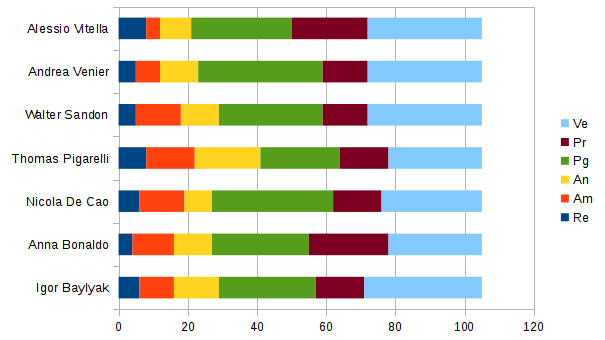
\includegraphics[width=\textwidth]{../img/diagrammaBarreRiepilogoRotazioneRuoli.png}
		\caption{Diagramma della rotazione dei ruoli - Riepilogo}
	\end{figure}
\end{center}

\newpage
\subsubsection{Prospetto economico}
Qui viene proposto il sommario dei costi per periodo durante tutta la durata del progetto didattico previsto.

\begin{table}[H]
	\begin{center}
		\begin{tabular}{l r r}
			\toprule
			\textbf{Ruolo}	& \textbf{Ore} & \textbf{Costo (\euro)} \\ \midrule
			\midrule
			\FA{} & 161 & 3 455.00 \\ \midrule
			\FAD{} & 30 & 650.00 \\ \midrule
			\FPA{} & 79 & 1 598.00 \\ \midrule
			\FPD{} & 136 & 2 800.00 \\ \midrule
			\FPDC{} & 203 & 3 453.00 \\ \midrule
			\FVV{} & 126 & 2 377.00 \\ \midrule
			\textbf{Totale} & \textbf{735} & \textbf{14 303.00} \\
			\bottomrule
		\end{tabular}
		\caption{Prospetto economico - Sommario}
	\end{center}
\end{table}

Nella tabella seguente sono riportate le ore di lavoro previste ed il loro costo per ogni ruolo durante tutta la fare del progetto didattico previsto.

\begin{table}[H]
	\begin{center}
		\begin{tabular}{l r c r}
			\toprule
			\textbf{Ruolo}	& \textbf{Ore} & \textbf{Costo (\euro/ora)}	& \textbf{Costo (\euro)} \\ \midrule
			\midrule
			\RE{} & 42 & 30 & 1 260.00 \\ \midrule
			\AM{} & 73 & 20 & 1 460.00 \\ \midrule
			\AN{} & 82 & 25 & 2 050.00 \\ \midrule
			\PG{} & 209 & 22 & 4 598.00 \\ \midrule
			\PR{} & 113 & 15 & 1 695.00 \\ \midrule
			\VR{} & 216 & 15 & 3 240.00 \\ \midrule
			\textbf{Totale} & \textbf{735} &  & \textbf{14 303.00} \\
			\bottomrule
		\end{tabular}
		\caption{Prospetto economico - Sommario}
	\end{center}
\end{table}

\begin{center}
	\begin{figure}[H]
		\centering 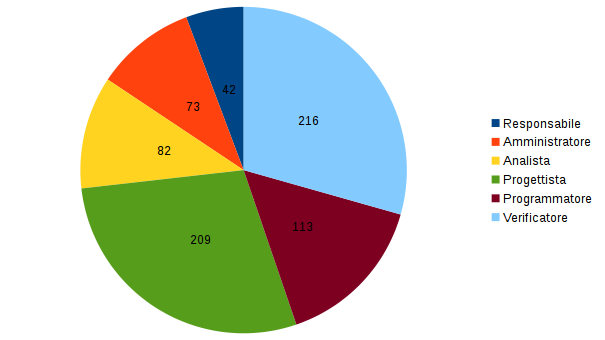
\includegraphics[width=\textwidth]{../img/diagrammaTortaRiepilogoTotaleOre.png}
		\caption{Diagramma della rotazione dei ruoli - Riepilogo}
	\end{figure}
\end{center}

\newpage
\subsection{Dettaglio fasi}

\subsubsection{Analisi}

\subsubsubsection{Rotazione dei ruoli}
Nella tabella seguente sono riportate le ore di lavoro previste per ogni membro del gruppo durante il periodo di \FA.

\begin{table}[H]
	\begin{center}
		\begin{tabular}{l r r r r r r r}
			\toprule
			\textbf{Membro}	&	\textbf{Re}	&	\textbf{Am}	& \textbf{An} & \textbf{Pg} & \textbf{Pr} & \textbf{Ve} & \textbf{Totale}\\
			\midrule
			\midrule
			\IB{} & 6 & 2 & 8 & & & 7 & 23 \\
			\midrule
			\AB{} & & 6 & 11 & & & 6 & 23 \\
			\midrule
			\NDC{} & 6 & 7 & 3 & & & 7 & 23 \\
			\midrule
			\TP{} & & 6 & 11 & & & 6 & 23 \\
			\midrule
			\WS{} & & 6 & 11 & & & 6 & 23 \\
			\midrule
			\AVE{} & & 7 & 11 & & & 5 & 23 \\
			\midrule
			\AVI{} & & 4 & 9 & & & 10 & 23 \\
			\bottomrule
		\end{tabular}
		\caption{Rotazione dei ruoli - \FA{}}
	\end{center}
\end{table}

\begin{center}
	\begin{figure}[H]
		\centering
		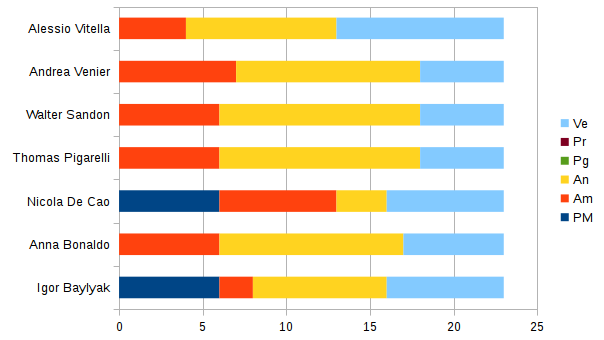
\includegraphics[width=\textwidth]{../img/diagrammaBarreAnalisiRotazioneRuoli.png}
		\caption{Diagramma della rotazione dei ruoli - \FA{}}
	\end{figure}
\end{center}

\newpage
\subsubsubsection{Prospetto economico}
Nella tabella seguente sono riportate le ore di lavoro previste ed il loro costo per ogni ruolo durante il periodo di \FA.

\begin{table}[H]
	\begin{center}
		\begin{tabular}{l r c r}
			\toprule
			\textbf{Ruolo}	& \textbf{Ore} & \textbf{Costo (\euro/ora)}	& \textbf{Costo (\euro)} \\
			\midrule
			\midrule
			\RE{} & 12 & 30 & 360.00\\
			\midrule
			\AM{} & 38 & 20 & 760.00\\ 
			\midrule
			\AN{} & 64 & 25 & 1 600.00\\ 
			\midrule
			\PG{} & & 22 & 0.00\\ 
			\midrule
			\PR{} & & 15 & 0.00\\ 
			\midrule
			\VR{} & 47 & 15 & 705.00\\ 
			\midrule
			\textbf{Totale} & \textbf{161} &  & \textbf{3 425.00}\\
			\bottomrule
		\end{tabular}
		\caption{Ripartizione oraria dei ruoli - \FA{}}
	\end{center}
\end{table}

\begin{center}
	\begin{figure}[H]
		\centering
		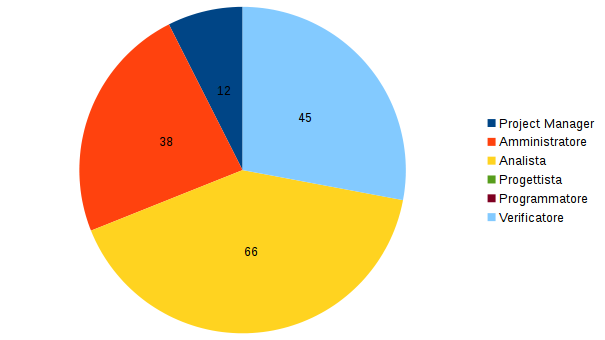
\includegraphics[width=\textwidth]{../img/diagrammaTortaAnalisiTotaleOre.png}
		\caption{Diagramma della ripartizione oraria dei ruoli - \FA{}}
	\end{figure}
\end{center}

\newpage
\subsubsection{Analisi di Dettaglio}

\subsubsubsection{Rotazione dei ruoli}
Nella tabella seguente sono riportate le ore di lavoro previste per ogni membro del gruppo durante il periodo di \FAD{}.

\begin{table}[H]
	\begin{center}
		\begin{tabular}{l r r r r r r r}
			\toprule
			\textbf{Membro}	&	\textbf{Re}	&	\textbf{Am}	& \textbf{An} & \textbf{Pg} & \textbf{Pr} & \textbf{Ve} & \textbf{Totale}\\
			\midrule
			\midrule
			\IB{} & & & 5 & & & & 5 \\
			\midrule
			\AB{} & 2 & & & & & & 2 \\
			\midrule
			\NDC{} & & & 5 & & & & 5 \\
			\midrule
			\TP{} & & 8 & & & & & 8 \\
			\midrule
			\WS{} & & & & & & 2 & 2 \\
			\midrule
			\AVE{} & & & & & & 2 & 2 \\
			\midrule
			\AVI{} & & & & & & 2 & 2 \\
			\bottomrule
		\end{tabular}
		\caption{Rotazione dei ruoli - \FAD{}}
	\end{center}
\end{table}

\begin{center}
	\begin{figure}[H]
		\centering	
		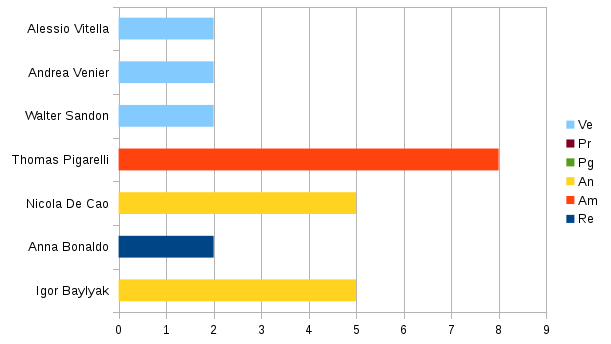
\includegraphics[width=\textwidth]{../img/diagrammaBarreAnalisiDiDettaglioRotazioneRuoli.png}
		\caption{Diagramma della rotazione dei ruoli - \FAD{}}
	\end{figure}
\end{center}

\newpage
\subsubsubsection{Prospetto economico}
Nella tabella seguente sono riportate le ore di lavoro previste ed il loro costo per ogni ruolo durante il periodo di \FAD{}.

\begin{table}[H]
	\begin{center}
		\begin{tabular}{l r c r}
			\toprule
			\textbf{Ruolo}	& \textbf{Ore} & \textbf{Costo (\euro/ora)}	& \textbf{Costo (\euro)} \\ \midrule
			\midrule
			\RE{} & 2 & 30 & 60.00 \\ \midrule
			\AM{} & 8 & 20 & 160.00 \\ \midrule
			\AN{} & 10 & 25 & 250.00 \\ \midrule
			\PG{} & & 22 & 0.00 \\ \midrule
			\PR{} & & 15 & 0.00 \\ \midrule
			\VR{} & 6 & 15 & 90.00 \\ \midrule
			\textbf{Totale} & \textbf{26} &  & \textbf{560.00} \\
			\bottomrule
		\end{tabular}
		\caption{Prospetto economico - \FAD{}}
	\end{center}
\end{table}

\begin{center}
	\begin{figure}[H]
		\centering 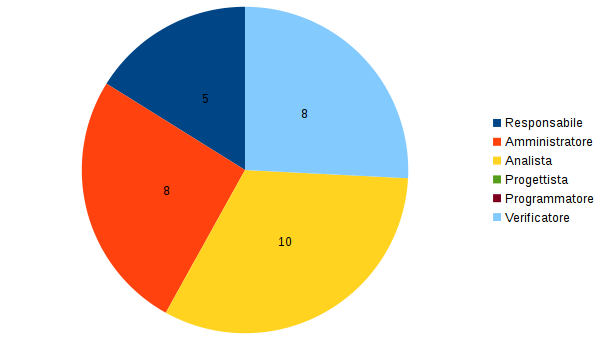
\includegraphics[width=\textwidth]{../img/diagrammaTortaAnalisiDiDettaglioTotaleOre.png}
		\caption{Diagramma della ripartizione oraria dei ruoli - \FAD{}}
	\end{figure}
\end{center}

\newpage
\subsubsection{Progettazione Architetturale}

\subsubsubsection{Rotazione dei ruoli}
Nella tabella seguente sono riportate le ore di lavoro previste per ogni membro del gruppo durante il periodo di \FP.

\begin{table}[H]
	\begin{center}
		\begin{tabular}{l r r r r r r r}
			\toprule
			\textbf{Membro}	&	\textbf{Re}	&	\textbf{Am}	& \textbf{An} & \textbf{Pg} & \textbf{Pr} & \textbf{Ve} & \textbf{Totale}\\
			\midrule
			\midrule
			\IB{} & & & & 8 & & 3 & 11 \\
			\midrule
			\AB{} & 2 & & & 8 & & 3 & 13 \\
			\midrule
			\NDC{} & & & & 8 & & 3 & 11 \\
			\midrule
			\TP{} & & & & 8 & & & 8 \\
			\midrule
			\WS{} & & & & 9 & & 3 & 12 \\
			\midrule
			\AVE{} & & & & 9 & & 4 & 13 \\
			\midrule
			\AVI{} & & & & 9 & & 4 & 13 \\
			\bottomrule
		\end{tabular}
		\caption{Rotazione dei ruoli - \FPA{}}
	\end{center}
\end{table}

\begin{center}
	\begin{figure}[H]
		\centering 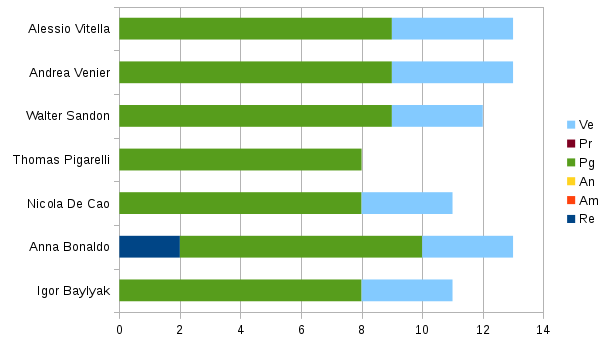
\includegraphics[width=\textwidth]{../img/diagrammaBarreProgettazioneArchitetturaleRotazioneRuoli.png}
		\caption{Diagramma della rotazione dei ruoli - \FPA{}}
	\end{figure}
\end{center}

\newpage
\subsubsubsection{Prospetto economico}
Nella tabella seguente sono riportate le ore di lavoro previste ed il loro costo per ogni ruolo durante il periodo di \FP.

\begin{table}[H]
	\begin{center}
		\begin{tabular}{l r c r}
			\toprule
			\textbf{Ruolo}	& \textbf{Ore} & \textbf{Costo (\euro/ora)}	& \textbf{Costo (\euro)} \\ \midrule
			\midrule
			\RE{} & 2 & 30 & 60.00 \\ \midrule
			\AM{} & & 20 & 0.00 \\ \midrule
			\AN{} & & 25 & 0.00 \\ \midrule
			\PG{} & 59 & 22 & 1 298.00 \\ \midrule
			\PR{} & & 15 & 0.00 \\ \midrule
			\VR{} & 20 & 15 & 300.00 \\ \midrule
			\textbf{Totale} & \textbf{81} &  & \textbf{1 658.00} \\
			\bottomrule
		\end{tabular}
		\caption{Prospetto economico - \FPA{}}
	\end{center}
\end{table}

\begin{center}
	\begin{figure}[H]
		\centering	
	    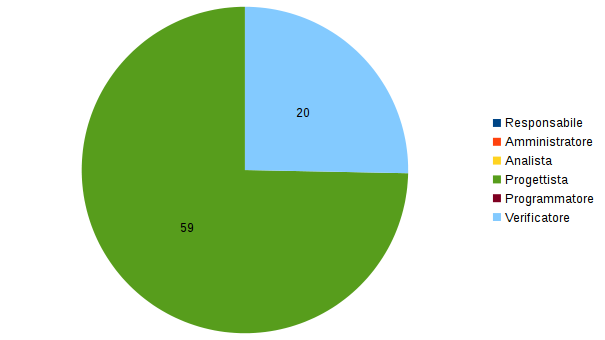
\includegraphics[width=\textwidth]{../img/diagrammaTortaProgettazioneArchitetturaleTotaleOre.png}
		\caption{Diagramma della ripartizione oraria dei ruoli - \FPA{}}
	\end{figure}
\end{center}

\newpage
\subsubsection{Progettazione di Dettaglio}

\subsubsubsection{Rotazione dei ruoli}
Nella tabella seguente sono riportate le ore di lavoro previste per ogni membro del gruppo durante il periodo di \FPD{}.

\begin{table}[H]
	\begin{center}
		\begin{tabular}{l r r r r r r r}
			\toprule
			\textbf{Membro}	&	\textbf{Re}	&	\textbf{Am}	& \textbf{An} & \textbf{Pg} & \textbf{Pr} & \textbf{Ve} & \textbf{Totale}\\
			\midrule
			\midrule
			\IB{} & & & & 15 & & 4 & 19 \\
			\midrule
			\AB{} & & & & 15 & & 5 & 20 \\
			\midrule
			\NDC{} & & & & 15 & & 4 & 19 \\
			\midrule
			\TP{} & 4 & & & 15 & & & 19 \\
			\midrule
			\WS{} & & & & 14 & & 7 & 21 \\
			\midrule
			\AVE{} & & & & 14 & & 6 & 20 \\
			\midrule
			\AVI{} & & & & 12 & & 8 & 20 \\
			\bottomrule
		\end{tabular}
		\caption{Rotazione dei ruoli - \FPD{}}
	\end{center}
\end{table}

\begin{center}
	\begin{figure}[H]
		\centering	
        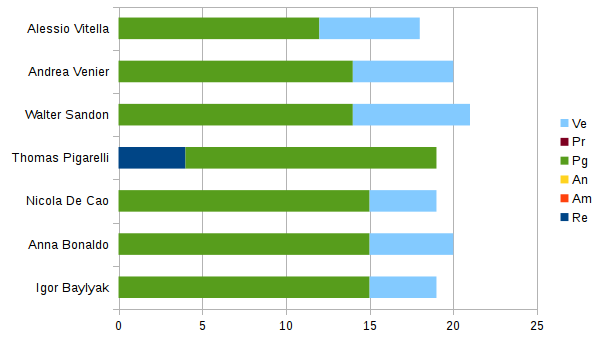
\includegraphics[width=\textwidth]{../img/diagrammaBarreProgettazioneDiDettaglioRotazioneRuoli.png}
		\caption{Diagramma della rotazione dei ruoli - \FPD{}}
	\end{figure}
\end{center}

\newpage
\subsubsubsection{Prospetto economico}
Nella tabella seguente sono riportate le ore di lavoro previste ed il loro costo per ogni ruolo durante il periodo di \FPD{}.

\begin{table}[H]
	\begin{center}
		\begin{tabular}{l r c r}
			\toprule
			\textbf{Ruolo}	& \textbf{Ore} & \textbf{Costo (\euro/ora)}	& \textbf{Costo (\euro)} \\ \midrule
			\midrule
			\RE{} & 4 & 30 & 120.00 \\ \midrule
			\AM{} & & 20 & 0.00 \\ \midrule
			\AN{} & & 25 & 0.00 \\ \midrule
			\PG{} & 100 & 22 & 2 200.00 \\ \midrule
			\PR{} & & 15 & 0.00 \\ \midrule
			\VR{} & 34 & 15 & 510.00 \\ \midrule
			\textbf{Totale} & \textbf{138} &  & \textbf{2 830.00} \\
			\bottomrule
		\end{tabular}
		\caption{Prospetto economico - \FPD{}}
	\end{center}
\end{table}

\begin{center}
	\begin{figure}[H]
		\centering	
        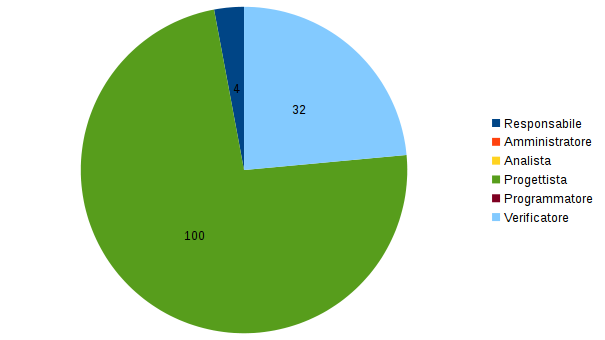
\includegraphics[width=\textwidth]{../img/diagrammaTortaProgettazioneDiDettaglioTotaleOre.png}
		\caption{Diagramma della ripartizione oraria dei ruoli - \FPD{}}
	\end{figure}
\end{center}

\newpage
\subsubsection{Codifica}

\subsubsubsection{Rotazione dei Ruoli}
Nella tabella seguente sono riportate le ore di lavoro previste per ogni membro del gruppo durante il periodo di \FC.

\begin{table}[H]
	\begin{center}
		\begin{tabular}{l r r r r r r r}
			\toprule
			\textbf{Membro}	&	\textbf{Re}	&	\textbf{Am}	& \textbf{An} & \textbf{Pg} & \textbf{Pr} & \textbf{Ve} & \textbf{Totale}\\
			\midrule
			\midrule
			\IB{} & & & & 5 & 14 & 10 & 29 \\
			\midrule
			\AB{} & & & & 5 & 14 & 10 & 29 \\
			\midrule
			\NDC{} & & & & 6 & 14 & 9 & 29 \\
			\midrule
			\TP{} & & & 8 & & 14 & 7 & 29 \\
			\midrule
			\WS{} & 3 & 7 & & & 13 & 6 & 29 \\
			\midrule
			\AVE{} & 3 & & & 5 & 13 & 8 & 29 \\
			\midrule
			\AVI{} & & & & 8 & 13 & 8 & 29 \\
			\bottomrule
		\end{tabular}
		\caption{Rotazione dei ruoli - \FPDC{}}
	\end{center}
\end{table}

\begin{center}
	\begin{figure}[H]
		\centering		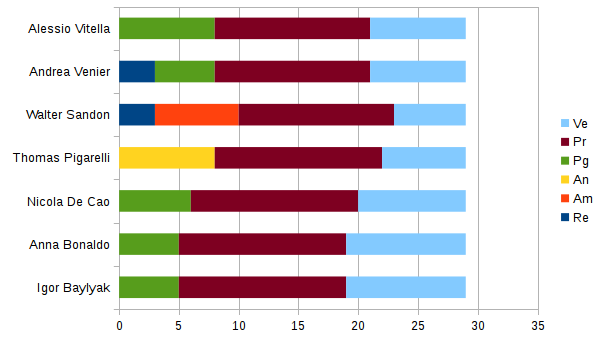
\includegraphics[width=\textwidth]{../img/diagrammaBarreCodificaRotazioneRuoli.png}
		\caption{Diagramma della rotazione dei ruoli - \FPDC{}}
	\end{figure}
\end{center}

\newpage
\subsubsubsection{Prospetto economico}
Nella tabella seguente sono riportate le ore di lavoro previste ed il loro costo per ogni ruolo durante il periodo di \FC.

\begin{table}[H]
	\begin{center}
		\begin{tabular}{l r c r}
			\toprule
			\textbf{Ruolo}	& \textbf{Ore} & \textbf{Costo (\euro/ora)}	& \textbf{Costo (\euro)} \\ \midrule
			\midrule
			\RE{} & 6 & 30 & 180.00 \\ \midrule
			\AM{} & 7 & 20 & 140.00 \\ \midrule
			\AN{} & 8 & 25 & 200.00 \\ \midrule
			\PG{} & 29 & 22 & 638.00 \\ \midrule
			\PR{} & 95 & 15 & 1 425.00 \\ \midrule
			\VR{} & 58 & 15 & 870.00 \\ \midrule
			\textbf{Totale} & \textbf{203} &  & \textbf{3 453.00} \\
			\bottomrule
		\end{tabular}
		\caption{Prospetto economico - \FPDC{}}
	\end{center}
\end{table}

\begin{center}
	\begin{figure}[H]
		\centering
		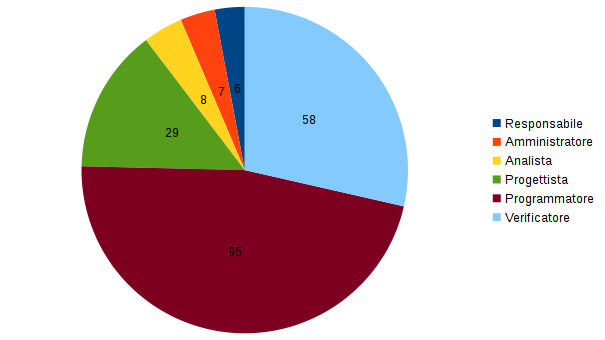
\includegraphics[width=\textwidth]{../img/diagrammaTortaCodificaTotaleOre.png}
		\caption{Diagramma della ripartizione oraria dei ruoli - \FPDC{}}
	\end{figure}
\end{center}

\newpage
\subsubsection{Validazione}

\subsubsubsection{Rotazione dei Ruoli}
Nella tabella seguente sono riportate le ore di lavoro previste per ogni membro del gruppo durante il periodo di \FV.

\begin{table}[H]
	\begin{center}
		\begin{tabular}{l r r r r r r r}
			\toprule
			\textbf{Membro}	&	\textbf{Re}	&	\textbf{Am}	& \textbf{An} & \textbf{Pg} & \textbf{Pr} & \textbf{Ve} & \textbf{Totale}\\
			\midrule
			\midrule
			\IB{} & & 8 & & & & 10 & 18 \\
			\midrule
			\AB{} & & 6 & & & 9 & 3 & 18 \\
			\midrule
			\NDC{} & & 6 & & 6 & & 6 & 18 \\
			\midrule
			\TP{} & 4 & & & & &14 & 18 \\
			\midrule
			\WS{} & 2 & & & 7 & & 9 & 18 \\
			\midrule
			\AVE{} & 2 & & & 8 & & 8 & 18 \\
			\midrule
			\AVI{} & 8 & & & & 9 & 1 & 18 \\
			\bottomrule
		\end{tabular}
		\caption{Rotazione dei ruoli - \FVV{}}
	\end{center}
\end{table}

\begin{center}
	\begin{figure}[H]
		\centering
		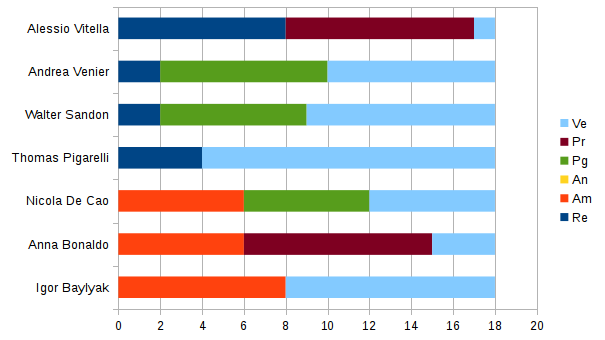
\includegraphics[width=\textwidth]{../img/diagrammaBarreVerificaValidazioneRotazioneRuoli.png}
		\caption{Diagramma della ripartizione oraria dei ruoli - \FVV{}}
	\end{figure}
\end{center}

\newpage
\subsubsubsection{Prospetto economico}
Nella tabella seguente sono riportate le ore di lavoro previste ed il loro costo per ogni ruolo durante il periodo di \FV.

\begin{table}[H]
	\begin{center}
		\begin{tabular}{l r c r}
			\toprule
			\textbf{Ruolo}	& \textbf{Ore} & \textbf{Costo (\euro/ora)}	& \textbf{Costo (\euro)} \\
			\midrule
			\midrule
			\RE{} & 16 & 30 & 480.00\\
			\midrule
			\AM{} & 20 & 20 & 400.00\\ 
			\midrule
			\AN{} & & 25 & 0.00\\ 
			\midrule
			\PG{} & 21 & 22 & 462.00\\ 
			\midrule
			\PR{} & 18 & 15 & 270.00\\ 
			\midrule
			\VR{} & 51 & 15 & 765.00\\ 
			\midrule
			\textbf{Totale} & \textbf{126} &  & \textbf{2 377.00}\\
			\bottomrule
		\end{tabular}
		\caption{Ripartizione oraria dei ruoli - \FVV{}}
	\end{center}
\end{table}

\begin{center}
	\begin{figure}[H]
		\centering
		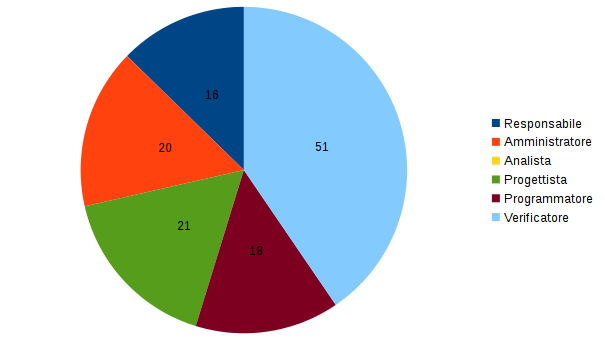
\includegraphics[width=\textwidth]{../img/diagrammaTortaVerificaValidazioneTotaleOre.png}
		\caption{Diagramma della ripartizione oraria dei ruoli - \FVV{}}
	\end{figure}
\end{center}

\newpage
\section{Consuntivo e preventivo a finire}

\subsection{Analisi}
Verrà mostrato il prospetto economico delle spese che effettivamente sono state sostenute rispetto alle ore preventivate.

\subsubsection{Rotazione dei Ruoli}
Nella tabella seguente sono riportate le differenze tra le ore di lavoro previste per ogni membro del gruppo con quelle realmente impiegate.

\begin{table}[H]
	\begin{center}
		\begin{tabular}{l r r r r r r r}
			\toprule
			\textbf{Membro}	&	\textbf{Re}	&	\textbf{Am}	& \textbf{An} & \textbf{Pg} & \textbf{Pr} & \textbf{Ve} & \textbf{Totale}\\
			\midrule
			\midrule
			\IB{} & 5(-1) & 2(0) & 9(+1) & & & 7(0) & 23(0) \\
			\midrule
			\AB{} & & 6(0) & 11(0) & & & 6(0) & 23(0) \\
			\midrule
			\NDC{} & 8(+2) & 7(0) & 2(-1) & & & 6(-1) & 23(0) \\
			\midrule
			\TP{} & & 6(0) & 9(-2) & & & 8(+2) & 23(0) \\
			\midrule
			\WS{} & & 7(+1) & 10(-1) & & & 6(0) & 23(0) \\
			\midrule
			\AVE{} & & 7(0) & 11(0) & & & 5(0) & 23(0) \\
			\midrule
			\AVI{} & & 4(0) & 8(-1) & & & 11(+1) & 23(0) \\
			\bottomrule
		\end{tabular}
		\caption{Rotazione dei ruoli effettive - \FA{}}
	\end{center}
\end{table}

\subsubsection{Prospetto economico}
Nella tabella seguente sono riportate le differenze tra le ore di lavoro previste ed il loro costo per ogni ruolo con quelle realmente impiegate.

\begin{table}[H]
	\begin{center}
		\begin{tabular}{l r c r}
			\toprule
			\textbf{Ruolo}	& \textbf{Ore} & \textbf{Costo (\euro/ora)}	& \textbf{Costo (\euro)} \\
			\midrule
			\midrule
			\RE{} & 13(+1) & 30.00 & 390.00(+30.00)\\
			\midrule
			\AM{} & 39(+1) & 20.00 & 780.00(+20.00)\\ 
			\midrule
			\AN{} & 60(-4) & 25.00 & 1 500.00(-100.00)\\ 
			\midrule
			\PG{} & & 22.00 & 0.00\\ 
			\midrule
			\PR{} & & 15.00 & 0.00\\ 
			\midrule
			\VR{} & 49(+2) & 15.00 & 735.00(+30.00)\\ 
			\midrule
			\midrule
			\textbf{Totale effettivo} & \textbf{161} &  & \textbf{3 405.00}\\
			\midrule
			\textbf{Totale preventivo} & \textbf{161} &  & \textbf{3 425.00}\\
			\midrule
			\textbf{Differenza} & \textbf{0} &  & \textbf{-20.00}\\
			\bottomrule
		\end{tabular}
		\caption{Ripartizione oraria dei ruoli effettivi - \FA{}}
	\end{center}
\end{table}

\begin{center}
	\begin{figure}[H]
		\centering
		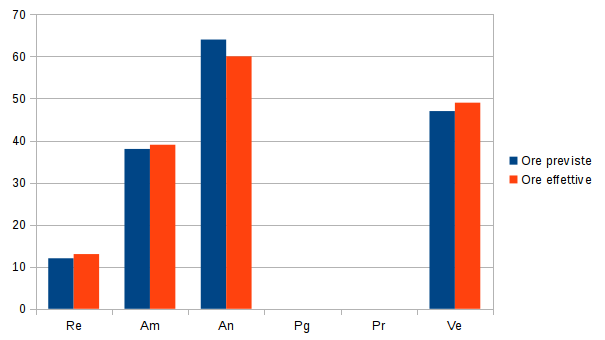
\includegraphics[width=\textwidth]{../img/diagrammaBarreAnalisiConsuntivo.png}
		\caption{Diagramma della ripartizione oraria dei ruoli effettiva - \FA{}}
	\end{figure}
\end{center}

\subsubsection{Conclusioni}
Il gruppo ha cercato di rispettare le ore previste con qualche aggiustamento e cambi di ruoli non previsti si è riusciti a mantenere le ore totali preventivate. Le ore per i differenti \mglspl{ruolo} sono state effettivamente diverse e hanno portato ad un deficit del bilancio di \euro{}-20.00.

\subsubsection{Preventivo a finire}
\label{sec:paf-analisi}
Dato che il consuntivo soprastante evidenzia un bilancio in deficit, è possibile impiegare il budget risparmiato nella periodo temporale successivo. In particolare i \euro{}20.00 risparmiati possono essere impiegati per aumentare le ore di verifica dei documenti corretti in seguito alla \RR{}.

\newpage

\subsection{Analisi di Dettaglio}
Verrà mostrato il prospetto economico delle spese che effettivamente sono state sostenute rispetto alle ore preventivate.

\subsubsection{Rotazione dei Ruoli}
Nella tabella seguente sono riportate le differenze tra le ore di lavoro previste per ogni membro del gruppo con quelle realmente impiegate.

\begin{table}[H]
	\begin{center}
		\begin{tabular}{l r r r r r r r}
			\toprule
			\textbf{Membro}	&	\textbf{Re}	&	\textbf{Am}	& \textbf{An} & \textbf{Pg} & \textbf{Pr} & \textbf{Ve} & \textbf{Totale}\\
			\midrule
			\midrule
            \IB{} & & & 9(+4) & & & & 9(+4) \\
			\midrule
            \AB{} & 2(0) & & & & & & 2(0) \\
			\midrule
            \NDC{} & & & 9(+4) & & & & 9(+4) \\
			\midrule
            \TP{} & & 6(-2) & 4(+4) & & & & 10(+2) \\
			\midrule
            \WS{} & & & & & & 3(+1) & 3(+1) \\
			\midrule
            \AVE{} & & & & & & 4(+2) & 4(+2) \\
			\midrule
            \AVI{} & & & & & & 3(+1) & 3(+1) \\
			\bottomrule
		\end{tabular}
		\caption{Rotazione dei ruoli effettive - \FAD{}}
	\end{center}
\end{table}

\subsubsection{Prospetto economico}
Nella tabella seguente sono riportate le differenze tra le ore di lavoro previste ed il loro costo per ogni ruolo con quelle realmente impiegate.

\begin{table}[H]
	\begin{center}
		\begin{tabular}{l r c r}
			\toprule
			\textbf{Ruolo}	& \textbf{Ore} & \textbf{Costo (\euro/ora)}	& \textbf{Costo (\euro)} \\ \midrule
			\midrule
            \RE{} & 2(0) & 30 & 60.00(+0.00) \\ \midrule
            \AM{} & 6(-2) & 20 & 120.00(-40.00) \\ \midrule
            \AN{} & 22(+12) & 25 & 550.00(+300.00) \\ \midrule
			\PG{} & & 22 & 0.00 \\ \midrule
			\PR{} & & 15 & 0.00 \\ \midrule
            \VR{} & 10(+4) & 15 & 150.00(+60.00) \\ \midrule
            \textbf{Totale effettivo} & \textbf{40} &  & \textbf{880.00} \\ \midrule
			\textbf{Totale preventivo} & \textbf{26} &  & \textbf{560.00} \\ \midrule
			\textbf{Differenza} & \textbf{+14} &  & \textbf{+320.00} \\ \midrule
			\bottomrule
		\end{tabular}
		\caption{Ripartizione oraria dei ruoli effettivi - \FAD{}}
	\end{center}
\end{table}

\begin{center}
	\begin{figure}[H]
		\centering
		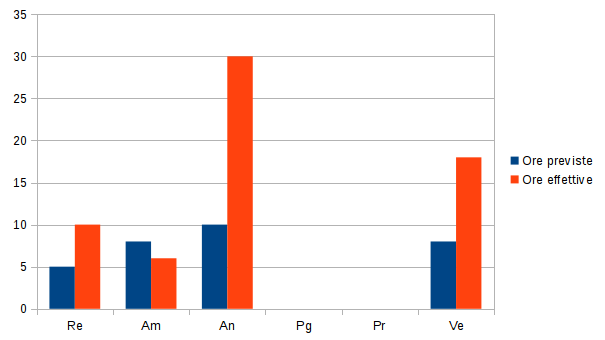
\includegraphics[width=\textwidth]{../img/diagrammaBarreAnalisiDiDettaglioConsuntivo.png}
		\caption{Diagramma della ripartizione oraria dei ruoli effettiva - \FAD{}}
	\end{figure}
\end{center}

\subsubsection{Conclusioni}
La correzione dei problemi rilevati dalla \RR{} hanno richiesto un maggior numero di ore rispetto a quelle preventivate. Questo non ha portato a ritardi rilevabili in quanto i membri del gruppo hanno lavorato in media un maggior numero di ore al giorno rispetto a quello preventivato. Tale numero aggiuntivo di ore ha riportato ad un incremento del costo per questo periodo pari ad \euro{}+320.00.

\subsubsection{Preventivo a finire}
La correzione dell'analisi ha permesso di semplificare notevolmente l'architettura e di ridurre il numero di requisiti obbligatori identificati nel periodo precedente.
Ci si aspetta quindi una semplificazione della stesura della \ST{} e della \DP{}, sperando che questo comporti una notevole riduzione dei costi nei prossimi due periodi. 

\newpage

\subsection{Progettazione architetturale}
Verrà mostrato il prospetto economico delle spese che effettivamente sono state sostenute rispetto alle ore preventivate.

\subsubsection{Rotazione dei Ruoli}
Nella tabella seguente sono riportate le differenze tra le ore di lavoro previste per ogni membro del gruppo con quelle realmente impiegate.

\begin{table}[H]
	\begin{center}
		\begin{tabular}{l r r r r r r r}
			\toprule
			\textbf{Membro}	&	\textbf{Re}	&	\textbf{Am}	& \textbf{An} & \textbf{Pg} & \textbf{Pr} & \textbf{Ve} & \textbf{Totale}\\
			\midrule
			\midrule
            \IB{} & & & & 8(0) & & 3(0) & 11(0) \\
			\midrule
            \AB{} & 2(0) & & & 6(-2) & & 3(0) & 11(-2) \\
			\midrule
            \NDC{} & & & & 8(0) & & 3(-1) & 11(-1) \\
			\midrule
            \TP{} & & & & 8(0) & & & 7(-1) \\
			\midrule
            \WS{} & & & & 6(-3) & & 3 & 9(-3) \\
			\midrule
            \AVE{} & & & & 7(-2) & & 3(-1) & 10(-3) \\
			\midrule
            \AVI{} & & & & 8(-1) & & 4(0) & 12(-1) \\
			\bottomrule
		\end{tabular}
		\caption{Rotazione dei ruoli effettive - \FPA{}}
	\end{center}
\end{table}

\subsubsection{Prospetto economico}
Nella tabella seguente sono riportate le differenze tra le ore di lavoro previste ed il loro costo per ogni ruolo con quelle realmente impiegate.

\begin{table}[H]
	\begin{center}
		\begin{tabular}{l r c r}
			\toprule
			\textbf{Ruolo}	& \textbf{Ore} & \textbf{Costo (\euro/ora)}	& \textbf{Costo (\euro)} \\ \midrule
			\midrule
            \RE{} & 6(+4) & 30 & 180.00(+120.00) \\ \midrule
			\AM{} & & 20 & 0.00 \\ \midrule
			\AN{} & & 25 & 0.00 \\ \midrule
            \PG{} & 49(-10) & 22 & 1 078.00(-220.00) \\ \midrule
			\PR{} & & 15 & 0.00 \\ \midrule
            \VR{} & 18(-2) & 15 & 270.00(-30.00) \\ \midrule
            \textbf{Totale effettivo} & \textbf{73} &  & \textbf{1 528.00} \\ \midrule
			\textbf{Totale preventivo} & \textbf{81} &  & \textbf{1 658.00} \\ \midrule
			\textbf{Differenza} & \textbf{-8} &  & \textbf{-130.00} \\ \midrule
			\bottomrule
		\end{tabular}
		\caption{Ripartizione oraria dei ruoli effettivi - \FPA{}}
	\end{center}
\end{table}

\begin{center}
	\begin{figure}[H]
		\centering
		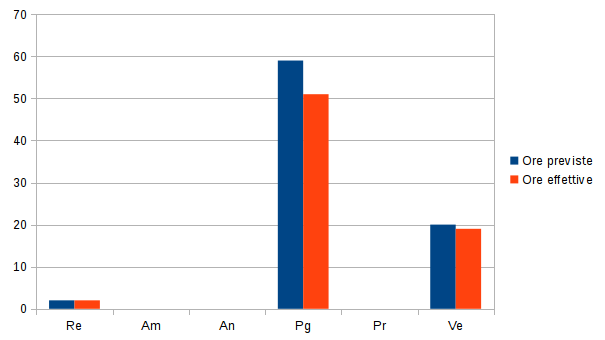
\includegraphics[width=\textwidth]{../img/diagrammaBarreProgettazioneArchitetturaleConsuntivo.png}
		\caption{Diagramma della ripartizione oraria dei ruoli effettiva - \FA{}}
	\end{figure}
\end{center}

\subsubsection{Conclusioni}
La rinegoziazione dei requisiti ha permesso una notevole semplificazione della progettazione ad alto livello portando ad una più semplice identificazione e successiva stesura dell'architettura. In totale, per questo periodo, si è riusciti a risparmiare un totale di \euro{}-130.00 che ci lasciano comunque in attivo di \euro{}+190.00 rispetto al consuntivo precedente.

\subsubsection{Preventivo a finire}
Ci si aspetta che la semplificazione dei requisiti continui, a cascata, a portare notevoli vantaggi nella stesura della \DP{} e della codifica stessa.

\newpage

\subsection{Progettazione di dettaglio}
Verrà mostrato il prospetto economico delle spese che effettivamente sono state sostenute rispetto alle ore preventivate.

\subsubsection{Rotazione dei Ruoli}
Nella tabella seguente sono riportate le differenze tra le ore di lavoro previste per ogni membro del gruppo con quelle realmente impiegate.

\begin{table}[H]
	\begin{center}
		\begin{tabular}{l r r r r r r r}
			\toprule
			\textbf{Membro}	&	\textbf{Re}	&	\textbf{Am}	& \textbf{An} & \textbf{Pg} & \textbf{Pr} & \textbf{Ve} & \textbf{Totale}\\
			\midrule
			\midrule
			\IB{} & & & & 13(-2) & & 3(-1) & 16(-3) \\
			\midrule
			\AB{} & & & & 13(-2) & & 4(-1) & 17(-3) \\
			\midrule
			\NDC{} & & & & 13(-2) & & 3(-1) & 16(-3) \\
			\midrule
			\TP{} & 10(+6) & & & 9(-6) & & & 19(0) \\
			\midrule
			\WS{} & & & & 13(-1) & & 5(-2) & 18(-3) \\
			\midrule
			\AVE{} & & & & 13(-1) & & 5(-1) & 18(-2) \\
			\midrule
			\AVI{} & & & & 11(-1) & & 7(-1) & 18(-2) \\
			\bottomrule
		\end{tabular}
		\caption{Rotazione dei ruoli effettive - \FPD{}}
	\end{center}
\end{table}

\subsubsection{Prospetto economico}
Nella tabella seguente sono riportate le differenze tra le ore di lavoro previste ed il loro costo per ogni ruolo con quelle realmente impiegate.

\begin{table}[H]
	\begin{center}
		\begin{tabular}{l r c r}
			\toprule
			\textbf{Ruolo}	& \textbf{Ore} & \textbf{Costo (\euro/ora)}	& \textbf{Costo (\euro)} \\ \midrule
			\midrule	
			\RE{} & 10(+6) & 30 & 300.00(+180.00) \\ \midrule
			\AM{} & & 20 & 0.00 \\ \midrule
			\AN{} & & 25 & 0.00 \\ \midrule
			\PG{} & 85(-15) & 22 & 1 870.00(-330.00) \\ \midrule
			\PR{} & & 15 & 0.00 \\ \midrule
			\VR{} & 27(-7) & 15 & 405.00(-105.00) \\ \midrule
            \textbf{Totale effettivo} & \textbf{122} &  & \textbf{2 575} \\ \midrule
			\textbf{Totale preventivo} & \textbf{138} &  & \textbf{2 830.00} \\ \midrule
			\textbf{Differenza} & \textbf{-16} &  & \textbf{-255.00} \\ \midrule
			\bottomrule
		\end{tabular}
		\caption{Ripartizione oraria dei ruoli effettivi - \FPD{}}
	\end{center}
\end{table}

\begin{center}
	\begin{figure}[H]
		\centering
		% 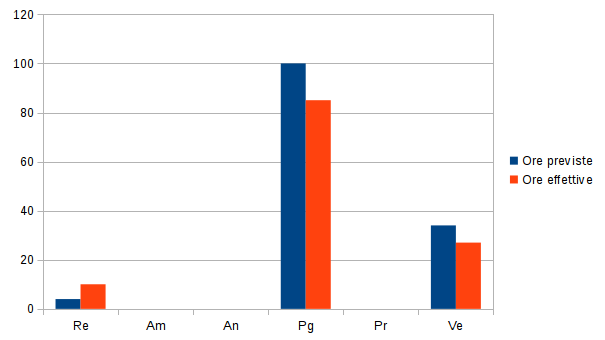
\includegraphics[width=\textwidth]{../img/diagrammaBarreProgettazioneDiDettaglioConsuntivo.png}
		\caption{Diagramma della ripartizione oraria dei ruoli effettiva - \FPD{}}
	\end{figure}
\end{center}

\subsubsection{Conclusioni}
Come previsto la semplificazione dei requisiti ha ridotto i costi della progettazione e relativa verifica. Nonostante anche in questo periodo di siano state più ore di lavoro per il \RE{} rispetto a quanto preventivato, il totale delle ore ha portato ad un deficit di \euro{}-255 che sommato al consuntivo dei due periodi precedenti risulta in \euro{}-65 che sommato al deficit del periodo di \FA{} risulta in un consuntivo di \euro{}-85.

\subsubsection{Preventivo a finire}
Dato il bilancio di \euro{}-85 e considerando che si prevedono anche notevoli semplificazioni anche nel periodo di \FC{}, sarà probabilmente possibile utilizzare il modello incrementale per concentrarsi anche su alcuni requisiti desiderabili o opzionali.

\newpage

\appendix
\section{Organigramma}

\subsection{Redazione}

\begin{table}[H]
	\begin{center}
		\begin{tabular}{l l l}
			\toprule
            \textbf{Nominativo}	& \textbf{Data} & \textbf{Firma} \\ \midrule
			\midrule
            \TP{} & 2016-01-21 & 
\includegraphics[width=6cm]{../img/firmaPigarelli.png} \\ \midrule
            \NDC{} & 2016-01-21 & 
\includegraphics[width=6cm]{../img/firmaDeCao.png} \\ \midrule
			\WS{} & 2016-01-21 & 
\includegraphics[width=6cm]{../img/firmaSandon.png} \\
			\bottomrule
		\end{tabular}
	\end{center}
\end{table}

\subsection{Approvazione}

\begin{table}[H]
	\begin{center}
		\begin{tabular}{l l l}
			\toprule
            \textbf{Nominativo}	& \textbf{Data} & \textbf{Firma} \\ \midrule
			\midrule
			\RE{} & 2016-01-21 & 
\includegraphics[width=6cm]{../img/firmaDeCao.png} \\ \midrule
			Docente &  & \\
		\end{tabular}
	\end{center}
\end{table}

\subsection{Accettazione dei componenti}

\begin{table}[H]
	\begin{center}
		\begin{tabular}{l l l}
			\toprule
            \textbf{Nominativo}	& \textbf{Data} & \textbf{Firma} \\ \midrule
			\midrule
			\AVI{} & 2016-01-21 & 
\includegraphics[width=6cm]{../img/firmaVitella.png} \\ \midrule
			\AVE{} & 2016-01-21 & 
\includegraphics[width=6cm]{../img/firmaVenier.png} \\ \midrule
			\AB{} & 2016-01-21 & 
\includegraphics[width=6cm]{../img/firmaBonaldo.png} \\ \midrule
            \IB{} & 2016-01-21 & 
\includegraphics[width=6cm]{../img/firmaBaylyak.png} \\ \midrule
            \NDC{} & 2016-01-21 & 
\includegraphics[width=6cm]{../img/firmaDeCao.png} \\ \midrule
			\TP{} & 2016-01-21 & 
\includegraphics[width=6cm]{../img/firmaPigarelli.png} \\ \midrule
			\WS{} & 2016-01-21 & 
\includegraphics[width=6cm]{../img/firmaSandon.png} \\
			\bottomrule
		\end{tabular}
	\end{center}
\end{table}

\subsection{Componenti}

\begin{table}[H]
	\begin{center}
		\begin{tabular}{l r l}
			\toprule
            \textbf{Nominativo}	& \textbf{Matricola} & \textbf{Email} \\ \midrule
			\midrule
			\AVI{} & 1070121 & alessio.vitella@gmail.com \\ \midrule
			\AVE{} & 1037258 & andrea.egna@gmail.com \\ \midrule
			\AB{} & 1068547 & annabonaldo92@gmail.com \\ \midrule
			\IB{} & 1029328 & ibaylyak@gmail.com \\ \midrule
			\NDC{} & 1069989 & nicola.decao@gmail.com \\ \midrule
			\TP{}  & 1031858 & tpigarelli@gmail.com \\ \midrule
			\WS{} & 1009138 & walter.sandon79@gmail.com \\
			\bottomrule
		\end{tabular}
	\end{center}
\end{table}

\subsection{Ruoli e costi}\label{ruoli e costi}

\begin{table}[H]
	\begin{center}
		\begin{tabular}{l r}
			\toprule
            \textbf{Ruolo}	& \textbf{Costo (\euro/ora)} \\ \midrule
			\midrule
            \RE{} & 30 \\ \midrule
            \AM{} & 20 \\ \midrule
            \AN{} & 25 \\ \midrule
            \PG{} & 22 \\ \midrule
            \PR{} & 15 \\ \midrule
            \VR{} & 15 \\
			\bottomrule
		\end{tabular}
	\end{center}
\end{table}

\end{document}
